% !TeX root = ../../Book3.tex
% 纲要标题：## 第24章*　Yamabe 问题与临界变分
% 纲要位置：几何学计划纲要.md，第 3122 行。
% 正文状态：初稿；尚未正式审核。

% 纲要内容开始
% 
% > 本章目标与证明范围：以共形标量曲率为贯穿问题，完整处理非正 Yamabe 情形及严格低于球面阈值时的紧性论证。正质量等完成一般正情形所需的深层输入明确外引，不把全部存在性挤进“典型结果”。
% 
% 纲要内容结束

\OptionalChapter{Yamabe 问题与临界变分}{g3:ch:24}
\BookChapterNumber{g3:ch:24}

\begin{chapterabstract}
	固定一个共形类，能否选出标量曲率为常数的度量？本章把这个问题写成带体积约束的临界变分问题，计算共形 Laplace 算子的协变公式与 Yamabe 泛函的一、二阶变分。非负弱极小点通过截断吸收、椭圆正则性和最大值原理恢复为光滑正因子。对于非正 Yamabe 常数，直接方法给出存在性，并证明固定体积后的唯一性；对于严格低于球面常数的情形，用近锐 Sobolev 不等式、范数分裂和能量缺陷估计完整证明极小化序列的强紧性。最后说明局部曲率、Green 函数和正质量如何提供严格不等式，准确引用一般存在性所需的深层结果，并以谱与球面模型辨别临界点、局部极小和全局极小。
\end{chapterabstract}

\begin{learninggoals}
	\begin{itemize}
		\item 在非负 Laplace 约定下计算共形标量曲率、体积与共形能量的变化。
		\item 区分 \(H^1\) 能量空间、高正则性空间中的正开集与单位体积约束，验证变分的可微性。
		\item 由第一特征函数识别共形类的符号，并完整证明临界非负弱解的光滑正性。
		\item 对负值和零值分别证明极小化序列紧性，建立非正情形的存在与规范体积唯一性。
		\item 计算临界气泡的尺度、低阶范数与球面能量，解释端点 Sobolev 嵌入失紧。
		\item 证明范数分裂、近锐 Sobolev 估计及严格球面阈值下的极小值实现。
		\item 说明 Aubin 型局部测试与 Schoen 的 Green 函数方法各解决哪些情形，核对所用正质量版本。
		\item 计算约束 Hessian，并用球面共形变化及长圆柱乘积区分存在性、稳定性与唯一性。
	\end{itemize}
\end{learninggoals}

在曲面上，标量曲率是 Gauss 曲率的两倍；在高维，标量曲率只是所有截面曲率的一项收缩。固定共形类后要求它为常数，是一个未知正函数满足的一条标量方程。这个问题称为\term[Yamabe wenti]{Yamabe 问题}[Yamabe problem]。\footnote{\OriginalHanName{山辺英彦}（やまべ ひでひこ，Hidehiko Yamabe，1923--1960），日本数学家，研究拓扑群与微分几何。}它不要求各个截面方向的曲率相等，因而比常截面曲率条件保留了更多几何自由。

\ProseParagraphBreak
第3章的共形变化公式把曲率条件化成非线性椭圆方程。第三编已经提供 Sobolev 空间、椭圆正则性、Banach 微分与约束变分，眼下的新障碍是临界指数：一列共形因子可以在越来越小的区域变得越来越高，保持总体积，却在弱极限中消失。局部的 Euclid 气泡显示了这种集中所需的确切能量；它恰等于圆球的 Yamabe 常数。

\ProseParagraphBreak
本章先从能量符号入手。非正情形不需要锐常数就能恢复强收敛，并可用最大值原理比较两个正解。随后把一般极小化序列分成弱极限与余项，证明只要极小值严格低于球面常数，任何质量损失都会违反极小性。最后，Aubin\footnote{Thierry Émilien Flavien Aubin（1942--2009），法国数学家，研究黎曼几何与非线性偏微分方程。}的局部测试和 Schoen 的整体构造负责取得这个严格不等号；正质量输入连同其维数、共形平坦及刚性条件在第24.5节列出。共形方程、球面模型与变分方法的原文组织可参看\cite[第2--4节]{LeeParker1987Yamabe}。

% !TeX root = ../../Book3.tex
% 纲要标题：### 24.1 Yamabe 问题的变分设置
% 纲要位置：几何学计划纲要.md，第 3126 行。
% 正文状态：初稿；尚未正式审核。

% 纲要内容开始
% 
% 本章不再首次建立通用非线性工具；它们的证明位置统一前移至第三编。
% 
% * 函数空间与变分方法
% * 固定共形类、正因子及体积约束
% * 弱极小点与光滑正解
% * 第一特征值、Yamabe 常数与唯一性
% 
% 纲要内容结束

\section{Yamabe 问题的变分设置}
\label{g3:sec:2401}

本章固定一个闭、连通、光滑的黎曼流形 \((M^n,g)\)，其中 \(n\ge3\)。闭表示紧且无边界；积分使用黎曼体积密度，所以不要求可定向。记
\[
	s_g=\operatorname{Scal}_g,\qquad
	a_n=\frac{4(n-1)}{n-2},\qquad p=\frac{2n}{n-2},\qquad
	\Delta_g=-\operatorname{div}_g\nabla.
\]
于是 \(\int_M v\Delta_gv\,\mu_g=\int_M|\mathrm dv|_g^2\,\mu_g\)。以下的曲率方程、极值比较与能量公式都使用这一非负 Laplace 约定。

\subsection{函数空间与变分方法}
\label{g3:subsec:2401:01}
第13.5节的 Banach 隐函数定理适合研究已知解附近的变化，第13.6节的复合与约束变分则负责把方程放进函数空间。本章先用能量寻找一个解，再在取得解后研究它的正则性与变分性质。这样做所需的空间有两种。

\ProseParagraphBreak
极小化采用实 Hilbert 空间 \(H^1(M)\)。由\cref{g3:thm:compact-bundle-sobolev,g3:thm:compact-bundle-rellich}，有
\[
	H^1(M)\longrightarrow L^p(M),\qquad
	H^1(M)\lhook\joinrel\longrightarrow L^q(M)\quad(1\le q<p),
\]
其中前一嵌入连续，后一嵌入紧。特别地，\(H^1\) 有界列能抽出在 \(L^2\) 中强收敛的子列，但单位 \(L^p\) 范数可能在弱极限中损失。这个端点差别正是临界变分的困难。

\ProseParagraphBreak
研究光滑正解的局部变化时，可选 \(r>n\) 并使用
\[
	\mathcal U_r=\{u\in W^{2,r}(M):\min_Mu>0\}.
\]
连续嵌入 \(W^{2,r}\to C^1\) 使它成为开集。由\cref{g3:thm:sobolev-composition-smooth}，在此集合上取实数幂、倒数及对数都是光滑的 Sobolev 复合。相应的曲率方程可作为到 \(L^r(M)\) 的光滑映射处理。\(H^1\) 中的非负锥则不是这样的开集：在一个小球中加入高度固定的负凸起，其 \(H^1\) 范数随球半径趋零，因为 \(n>2\)。因此不能把高正则性空间中的正开集直接搬到能量空间。

\subsection{固定共形类、正因子及体积约束}
\label{g3:subsec:2401:02}
\termidx[gongxing lei]{共形类}
\foreignidx{conformal class}
\begin{definition}\label{g3:def:yamabe-class-constraint}
	设 \((M^n,g)\) 为闭连通光滑黎曼流形，\(n\ge3\)。
	记 \(p=2n/(n-2)\)。
	\(g\) 的光滑共形类是
	\[
		[g]=\{u^{4/(n-2)}g:u\in C^\infty(M),\ u>0\}.
	\]
	对正因子 \(u\)，记 \(g_u=u^{4/(n-2)}g\)。体积变化为
	\[
		\mu_{g_u}=u^p\mu_g,\qquad
		\operatorname{Vol}(M,g_u)=\int_Mu^p\,\mu_g.
	\]
	在 \(H^1(M)\) 中相应采用约束 \(C(u)=\int_M|u|^p\,\mu_g=1\)。
\end{definition}
\symidx{\([g]\)：黎曼度量 \(g\) 的光滑共形类}

体积公式来自行列式：度量乘以 \(u^{4/(n-2)}\)，体积密度乘以它的 \(n/2\) 次方。每条正射线 \(\{tu:t>0\}\) 因而恰有一个单位体积代表 \(u/\|u\|_p\)。这只固定常数伸缩；对流形作共形自微分同胚仍可能产生不同的单位体积度量。

\begin{lemma}\label{g3:lem:yamabe-constraint-smoothness}
	设 \((M^n,g)\) 为闭连通光滑黎曼流形，\(n\ge3\)。
	记 \(p=2n/(n-2)\)。
	令 \(C(u)=\int_M|u|^p\,\mathrm d\mu_g\)，则 \(C:H^1(M)\to\mathbb R\) 为 \(C^2\) 映射，且
	\[
		\mathrm DC(u)h=p\int_M|u|^{p-2}uh\,\mu_g,\qquad
		\mathrm D^2C(u)[h,k]=p(p-1)\int_M|u|^{p-2}hk\,\mu_g.
	\]
	在 \(C(u)=1\) 处，其微分满射，约束切空间为
	\(\{h:\int_M|u|^{p-2}uh\,\mu_g=0\}\)。
\end{lemma}
\begin{proof}
	由 Hölder 不等式，三个因子 \(|u|^{p-2},h,k\) 的指数分别为 \(p/(p-2),p,p\)，所以第二式定义连续双线性型。映射 \(u\mapsto |u|^{p-2}\) 从 \(L^p\) 连续到 \(L^{p/(p-2)}\)：当 \(p-2\le1\) 时用幂函数的 Hölder 估计，当 \(p-2>1\) 时用中值公式和 Hölder 不等式。沿线段积分这个连续双线性型，先得到一阶微分的余项估计，再得到 \(C\) 的微分公式，故确为 Fréchet 二次连续可微。连续嵌入 \(H^1\to L^p\) 将结论限制到 \(H^1\)。最后 \(\mathrm DC(u)u=p\ne0\)，故微分满射；第13.5节的水平集定理给出所述切空间。
\end{proof}

这里没有要求 \(C\) 在 \(H^1\) 上无限次可微。临界指数可能不是整数，而约束乘子和二变分只需上述可微性。

\subsection{弱极小点与光滑正解}
\label{g3:subsec:2401:03}
先写出后续使用的解析量：
\begin{equation}\label{g3:eq:yamabe-energy-definition}
	L_g=a_n\Delta_g+s_g,\qquad
	E_g(u)=\int_M(a_n|\mathrm du|_g^2+s_gu^2)\,\mu_g,\qquad
	Q_g(u)=\frac{E_g(u)}{\|u\|_p^2}\quad(u\ne0).
\end{equation}
\symidx{\(L_g\)：共形 Laplace 算子 \(\frac{4(n-1)}{n-2}\Delta_g+s_g\)}
\symidx{\(Q_g\)：Yamabe 商}
\(L_g\) 称为\term[gongxing Laplace suanzi]{共形 Laplace 算子}[conformal Laplacian]。下一节将由曲率变化证明：\(Q_g(u)\) 正是 \(g_u\) 的规范化总标量曲率。它对 \(u\) 的常数倍不变，因此可以在 \(C=1\) 上最小化 \(E_g\)。

\begin{definition}\label{g3:def:yamabe-constant}
	设 \((M^n,g)\) 为闭连通光滑黎曼流形，\(n\ge3\)。
	对所用度量 \(h\)，记 \(E_h(v)=\int_M(\tfrac{4(n-1)}{n-2}|\mathrm dv|_h^2+s_hv^2)\,\mathrm d\mu_h\)，\(Q_h(v)=E_h(v)/\|v\|_{L^{2n/(n-2)}(h)}^2\)（\(v\ne0\)）。
	固定共形类的\term[Yamabe changshu]{Yamabe 常数}[Yamabe constant]定义为
	\[
		Y(M,[g])=\inf_{0\ne u\in H^1(M)}Q_g(u).
	\]
	\symidx{\(Y(M,[g])\)：共形类 \([g]\) 的 Yamabe 常数}
	本章简称 \(Y\)。这个量只对给定共形类取下确界；对所有共形类再取上确界是另一个不变量。
\end{definition}

\begin{proposition}\label{g3:prop:yamabe-admissible-density}
	设 \((M^n,g)\) 为闭连通光滑黎曼流形，\(n\ge3\)。记 \(Y=Y(M,[g])\) 为 \([g]\) 的 Yamabe 常数。
	\(Y\) 有限，并且其定义中的竞争者可以依次限制为非负 \(H^1\) 函数、光滑正函数，所得下确界不变。
\end{proposition}
\begin{proof}
	令 \(s_g^- =\max\{-s_g,0\}\)，由有限体积上的 Hölder 不等式，
	\[
		E_g(u)\ge a_n\|\mathrm du\|_2^2-\|s_g^-\|_\infty
		\operatorname{Vol}(M,g)^{2/n}\|u\|_p^2.
	\]
	所以 \(Y> -\infty\)；用 \(u=1\) 作竞争者又得有限上界。Sobolev 链式法则给出 \(|u|\in H^1\) 以及 \(|\mathrm d|u||=|\mathrm du|\) 几乎处处成立，故 \(Q_g(|u|)=Q_g(u)\)。这个等式在零水平集上使用了弱导数在那里几乎处处为零的性质，已在第11章的截断论证中建立。

	光滑函数在 \(H^1\) 中稠密，连续嵌入又使 \(L^p\) 范数收敛，因而 \(Q_g\) 在非零 \(H^1\) 函数上连续。对每个光滑实函数 \(v\)，取 \(v_\varepsilon=(v^2+\varepsilon^2)^{1/2}>0\)。它在 \(H^1\) 中趋于 \(|v|\)：导数是 \(v\,\mathrm dv/(v^2+\varepsilon^2)^{1/2}\)，由支配收敛及零水平集性质得到导数收敛。依次作光滑逼近和这一正化，就得到所需光滑正竞争者。
\end{proof}

极小值若在非零 \(H^1\) 函数处取得，先取绝对值、再规范体积，便得到非负的单位极小点。\Cref{g3:prop:constraint-lagrange-banach}随后产生弱 Euler 方程。将这个弱解恢复成光滑正函数，还需处理临界幂的可积性；\cref{g3:thm:yamabe-weak-regularity}将用截断和吸收先提高可积指数，再调用第12—13章的椭圆自举。这样，弱极小值才真正对应共形类中的光滑度量。

\subsection{第一特征值、Yamabe 常数与唯一性}
\label{g3:subsec:2401:04}
零阶函数 \(s_g\) 可以变号。决定共形类符号的量是整个二次型，而不只是某一点的标量曲率。考虑它的最低 Rayleigh 商
\[
	\lambda_1(L_g)=\inf_{v\ne0}\frac{E_g(v)}{\|v\|_2^2}.
\]
\begin{proposition}\label{g3:prop:yamabe-first-eigenvalue-sign}
	设 \((M^n,g)\) 为闭连通光滑黎曼流形，\(n\ge3\)。共形 Laplace 算子取 \(L_g=\tfrac{4(n-1)}{n-2}\Delta_g+s_g\)，其中 \(\Delta_g=-\operatorname{div}_g\nabla\)。记 \(Y=Y(M,[g])\) 为 \([g]\) 的 Yamabe 常数。
	\(L_g\) 有光滑严格正的第一特征函数 \(\phi\)，其特征空间为一维。\(Y\) 与 \(\lambda_1(L_g)\) 同号。特别地，\(Y=0\) 时 \(\ker L_g=\mathbb R\phi\)；\(Y>0\) 时核为零。
\end{proposition}
\begin{proof}
	在 \(\|v\|_2=1\) 上取极小化序列。零阶项有下界，所以导数范数有界；Rellich 紧性保留 \(L^2\) 约束，导数范数弱下半连续，故下确界取得。取绝对值后可设极小点非负，约束变分给出 \(L_g\phi=\lambda_1\phi\)。光滑系数椭圆正则性逐次提高 Sobolev 阶数，得到 \(\phi\) 光滑。写成 \(\Delta_g\phi=V\phi\)，其中 \(V=(\lambda_1-s_g)/a_n\) 有界。取 \(C\ge\max\{0,-\min V\}\)，令 \(w=-\phi\)，则
	\[
		(\operatorname{div}_g\nabla-C)w=(V+C)\phi\ge0.
	\]
	若 \(\phi\) 在某点为零，\(w\) 就在内部取得非负最大值零；\cref{g3:thm:strong-maximum-classical}及连通性迫使 \(\phi\equiv0\)，矛盾。因此 \(\phi>0\)。

	对光滑 \(v=\phi f\) 展开导数，并把交叉项与 \(|\mathrm d\phi|^2f^2\) 合为 \(\int\mathrm d\phi\cdot\mathrm d(\phi f^2)\)，得到
	\begin{equation}\label{g3:eq:yamabe-ground-state}
		E_g(v)=a_n\int_M\phi^2|\mathrm d(v/\phi)|^2\,\mu_g
		+\lambda_1\int_Mv^2\,\mu_g.
	\end{equation}
	\(\phi\) 有正下界，故公式由稠密性延至 \(H^1\)。任一第一特征函数使第一项为零，由连通性其与 \(\phi\) 的比为常数，得到单性。

	若 \(\lambda_1<0\)，以 \(\phi\) 测试即得 \(Y<0\)。若 \(\lambda_1=0\)，上式给出 \(E_g\ge0\) 且 \(E_g(\phi)=0\)，所以 \(Y=0\)，并同时识别核。若 \(\lambda_1>0\)，则 \(\|v\|_2^2\le E_g(v)/\lambda_1\)，而
	\[
		a_n\|\mathrm dv\|_2^2\le E_g(v)+\|s_g^-\|_\infty\|v\|_2^2.
	\]
	合并 Sobolev 不等式得 \(\|v\|_p^2\le C E_g(v)\)，故 \(Y\ge C^{-1}>0\)。三种情况穷尽全部可能。
\end{proof}

当 \(Y<0\) 时，零仍可能是 \(L_g\) 的较高特征值；负的最低特征值本身不蕴含算子可逆。另一方面，单位体积的非正 Yamabe 解将在\cref{g3:thm:yamabe-nonpositive-uniqueness}中证明唯一。这是非线性曲率方程的比较结论，与未加约束的线性算子是否有核是不同的问题。

\begin{example}\label{g3:exm:yamabe-flat-normalization}
	记 \(p=2n/(n-2)\)。记 \(a_n=4(n-1)/(n-2)\)。共形 Laplace 算子取 \(L_g=\tfrac{4(n-1)}{n-2}\Delta_g+s_g\)，\(\Delta_g=-\operatorname{div}_g\nabla\)。
	设 \((M^n,g)\) 为连通平坦环面，\(n\ge3\)。在此环面上 \(s_g=0\)，所以 \(L_g=a_n\Delta_g\)，其核由常数构成。共形因子 \(u=c>0\) 给出不同体积的平坦度量，而约束 \(c^p\operatorname{Vol}(M,g)=1\) 唯一确定 \(c\)。这里消除的是常数伸缩，连通性保证没有多个独立的常数方向。
\end{example}
% 纲要条目排为编号小节标题，并进入目录与书签；说明段仍保留于纲要注释中。

% !TeX root = ../../Book3.tex
% 纲要标题：### 24.2 共形变化与变分方程
% 纲要位置：几何学计划纲要.md，第 3135 行。
% 正文状态：初稿；尚未正式审核。

% 纲要内容开始
% 
% * n≥3 时标量曲率变换
% * 共形 Laplace 算子的协变性
% * Yamabe 泛函和临界指数
% * Euler–Lagrange 方程及正性
% 
% 纲要内容结束

\section{共形变化与变分方程}
\label{g3:sec:2402}

共形因子控制每一点的长度单位。标量曲率变化本来同时含有因子的一阶、二阶导数；选定幂次 \(4/(n-2)\) 后，一阶导数的平方项恰好抵消，留下一个线性椭圆算子与一个临界非线性幂。这是 Yamabe 问题可以用能量处理的原因。

\subsection{\texorpdfstring{\(n\ge3\) 时标量曲率变换}{n≥3 时标量曲率变换}}
\label{g3:subsec:2402:01}
第3.4节的\cref{g3:thm:conformal-curvature}已经从联络差计算曲率。为了核对这里使用的符号，令 \(\widehat g=e^{2f}g\)，重写其标量部分：
\[
	s_{\widehat g}=e^{-2f}\bigl(s_g+2(n-1)\Delta_gf
	-(n-1)(n-2)|\mathrm df|_g^2\bigr).
\]
现在取 \(f=2\log u/(n-2)\)。由于本书使用非负 Laplace 算子，链式公式为
\[
	\Delta_g\log u=u^{-1}\Delta_gu+u^{-2}|\mathrm du|_g^2.
\]
代入后，来自 \(\Delta_gf\) 和 \(|\mathrm df|^2\) 的平方项系数都为 \(4(n-1)/(n-2)\)，符号相反，遂得
\begin{equation}\label{g3:eq:yamabe-scalar-transformation}
	s_{g_u}=u^{-(p-1)}L_gu,
	\qquad L_g=a_n\Delta_g+s_g.
\end{equation}
这也就是\cref{g3:cor:conformal-scalar-power}在本章记号下的形式。要求 \(s_{g_u}=\lambda\) 为常数，等价于
\begin{equation}\label{g3:eq:yamabe-equation}
	L_gu=\lambda u^{p-1},\qquad u>0.
\end{equation}
其中 \(\lambda\) 也是未知量；只有选定体积或另一项规范化，才能消除常数伸缩。

\begin{example}
	记 \(p=2n/(n-2)\)。
	若 \(g\) 已有常标量曲率 \(s\)，取常因子 \(u=c>0\)，则
	\[
		s_{g_c}=s c^{-4/(n-2)},\qquad
		\operatorname{Vol}(g_c)=c^p\operatorname{Vol}(g).
	\]
	两式相乘得到 \(s_{g_c}\operatorname{Vol}(g_c)^{2/n}=s\operatorname{Vol}(g)^{2/n}\)。这提供了检验泛函幂次的一种直接方法。
\end{example}

\subsection{共形 Laplace 算子的协变性}
\label{g3:subsec:2402:02}
\begin{proposition}\label{g3:prop:conformal-laplacian-covariance}
	设 \((M^n,g)\) 为闭连通光滑黎曼流形，\(n\ge3\)。
	记 \(p=2n/(n-2)\)。共形 Laplace 算子取 \(L_g=\tfrac{4(n-1)}{n-2}\Delta_g+s_g\)，其中 \(\Delta_g=-\operatorname{div}_g\nabla\)。对所用度量 \(h\)，记 \(E_h(v)=\int_M(\tfrac{4(n-1)}{n-2}|\mathrm dv|_h^2+s_hv^2)\,\mathrm d\mu_h\)，\(Q_h(v)=E_h(v)/\|v\|_{L^{2n/(n-2)}(h)}^2\)（\(v\ne0\)）。
	设 \(u>0\) 光滑，\(\widehat g=u^{4/(n-2)}g\)。对任意光滑实函数 \(v\)，有
	\begin{equation}\label{g3:eq:conformal-laplacian-covariance}
		L_{\widehat g}v=u^{-(p-1)}L_g(uv).
	\end{equation}
	因此对 \(v\in H^1(M)\)，
	\begin{equation}\label{g3:eq:yamabe-conformal-energy}
		E_{\widehat g}(v)=E_g(uv),\qquad
		\|v\|_{L^p(\widehat g)}=\|uv\|_{L^p(g)},\qquad
		Q_{\widehat g}(v)=Q_g(uv).
	\end{equation}
	特别地，\(Y(M,[g])\) 与共形类代表的选择无关。
\end{proposition}
\begin{proof}
	先令 \(v>0\)。同一个度量既可以写成 \(v^{4/(n-2)}\widehat g\)，也可以写成 \((uv)^{4/(n-2)}g\)。分别对两次变化使用式\eqref{g3:eq:yamabe-scalar-transformation}，得到
	\[
		v^{-(p-1)}L_{\widehat g}v=(uv)^{-(p-1)}L_g(uv),
	\]
	于是得到协变公式。对一般光滑 \(v\)，取常数 \(A>\|v\|_\infty\)，把已证式分别用于 \(v+A\) 和 \(A\)，相减即得。

	分部积分并使用 \(\mu_{\widehat g}=u^p\mu_g\)，得
	\[
		\int_M vL_{\widehat g}v\,\mu_{\widehat g}
		=\int_MuvL_g(uv)\,\mu_g=E_g(uv).
	\]
	范数等式直接来自体积公式。乘以固定光滑正函数 \(u\) 是 \(H^1\) 的有界同构，故稠密性将等式延到 \(H^1\)，并在取下确界时给出竞争者之间的双射。
\end{proof}

有些文献把 \(L_g\) 除以 \(a_n\)，写成 \(\Delta_g+(n-2)s_g/[4(n-1)]\)；若还把 Laplace 算子的符号反转，微分项又变号。引用其方程或最佳常数时，需要同时换算二次型和乘子。本章固定 \(a_n\Delta_g+s_g\)，使解对应的乘子直接等于标量曲率。

\subsection{Yamabe 泛函和临界指数}
\label{g3:subsec:2402:03}
对任意度量 \(h\)，定义规范化总标量曲率
\[
	\mathcal S(h)=\frac{\int_Ms_h\,\mu_h}
	{\operatorname{Vol}(M,h)^{(n-2)/n}}.
\]
式\eqref{g3:eq:yamabe-scalar-transformation}和体积公式给出
\begin{equation}\label{g3:eq:yamabe-geometric-functional}
	\mathcal S(g_u)
	=\frac{\int_MuL_gu\,\mu_g}{(\int_Mu^p\,\mu_g)^{2/p}}
	=Q_g(u).
\end{equation}
因此 \(Q_g\) 称为\term[Yamabe fanhan]{Yamabe 泛函}[Yamabe functional]。由\cref{g3:prop:yamabe-admissible-density}，在光滑共形度量中取 \(\mathcal S\) 的下确界，等于在整个 \(H^1\) 中取 \(Q_g\) 的下确界。

\ProseParagraphBreak
临界指数 \(p\) 同时来自几何体积和分析缩放。对 \(\mathbb R^n\) 上的紧支函数设
\[
	v_\varepsilon(x)=\varepsilon^{-(n-2)/2}v(x/\varepsilon).
\]
换元 \(x=\varepsilon y\) 后，\(\int|\mathrm dv_\varepsilon|^2\) 和 \(\int|v_\varepsilon|^p\) 都不变，而 \(\int|v_\varepsilon|^q=\varepsilon^{n-q(n-2)/2}\int|v|^q\)。当 \(q<p\) 时，后一幂次为正；在 \(q=p\) 时，它正好消失。一团函数可以越缩越小，同时保留全部导数能量和临界范数。第24.4节会用达到锐 Sobolev 常数的气泡把这个现象定量化。

\begin{proposition}\label{g3:prop:yamabe-second-variation}
	设 \((M^n,g)\) 为闭连通光滑黎曼流形，\(n\ge3\)。
	记 \(p=2n/(n-2)\)。共形 Laplace 算子取 \(L_g=\tfrac{4(n-1)}{n-2}\Delta_g+s_g\)，其中 \(\Delta_g=-\operatorname{div}_g\nabla\)。对所用度量 \(h\)，记 \(E_h(v)=\int_M(\tfrac{4(n-1)}{n-2}|\mathrm dv|_h^2+s_hv^2)\,\mathrm d\mu_h\)，\(Q_h(v)=E_h(v)/\|v\|_{L^{2n/(n-2)}(h)}^2\)（\(v\ne0\)）。
	设 \(u>0\) 光滑、\(\int_Mu^p\,\mu_g=1\)，且 \(L_gu=\lambda u^{p-1}\)。若 \(h\in H^1(M)\) 满足 \(\int_Mu^{p-1}h\,\mu_g=0\)，则在该约束方向上的二变分为
	\begin{equation}\label{g3:eq:yamabe-second-variation}
		\mathrm D^2Q_g(u)[h,h]
		=2\left(E_g(h)-(p-1)\lambda\int_Mu^{p-2}h^2\,\mu_g\right).
	\end{equation}
	所以约束局部极小点必使括号中的二次型非负。
\end{proposition}
\begin{proof}
	由约束切向条件，\(C(u+th)=1+\tfrac12p(p-1)t^2\int u^{p-2}h^2+o(t^2)\)。另一方面，方程给出 \(E_g(u)=\lambda\) 与 \(\int hL_gu=0\)，故 \(E_g(u+th)=\lambda+t^2E_g(h)\)。把两式代入 \(Q=E C^{-2/p}\)，利用 \((1+x)^{-2/p}=1-(2/p)x+o(x)\)，比较 \(t^2\) 系数即得。曲线 \((u+th)/\|u+th\|_p\) 属于能量空间中的约束，且 \(Q\) 在常数伸缩下不变，因而此式也就是约束 Hessian。若只考虑光滑正竞争者，先取光滑 \(h\)，利用 \(u\) 的正下界；取光滑逼近 \(h_j\to h\) 后，以 \(h_j-u\int_Mu^{p-1}h_j\,\mu_g\) 修正，它们仍趋于 \(h\) 并保持切向条件，故必要非负性延到全部切向 \(H^1\) 方向。
\end{proof}

\subsection{Euler–Lagrange 方程及正性}
\label{g3:subsec:2402:04}
\begin{proposition}\label{g3:prop:yamabe-euler-lagrange}
	设 \((M^n,g)\) 为闭连通光滑黎曼流形，\(n\ge3\)。
	记 \(p=2n/(n-2)\)。记 \(a_n=4(n-1)/(n-2)\)，\(s_g=\operatorname{Scal}_g\)。记 \(Y=Y(M,[g])\) 为 \([g]\) 的 Yamabe 常数。
	若 \(u\ge0\)、\(\|u\|_p=1\) 为 \(Y\) 的极小点，则对每个 \(h\in H^1(M)\)，
	\begin{equation}\label{g3:eq:yamabe-weak-equation}
		\int_M(a_n\langle\mathrm du,\mathrm dh\rangle+s_guh)\,\mu_g
		=Y\int_Mu^{p-1}h\,\mu_g.
	\end{equation}
\end{proposition}
\begin{proof}
	\(E_g\) 是连续二次型，\cref{g3:lem:yamabe-constraint-smoothness}给出约束的满射微分。由\cref{g3:prop:constraint-lagrange-banach}，存在常数 \(\eta\) 使 \(\mathrm DE_g(u)=\eta\,\mathrm DC(u)\)。将系数吸收到 \(\lambda=\eta p/2\)，得到右端为 \(\lambda\int u^{p-1}h\) 的弱方程；取 \(h=u\)，由约束得 \(\lambda=E_g(u)=Y\)。所有积分均有定义，因为 \(u^{p-1}\in L^{p/(p-1)}\) 且 \(h\in L^p\)。极小点虽然非负，却仍是整个实约束上的极小点，所以可以使用任意实切向方向。
\end{proof}

\begin{theorem}\label{g3:thm:yamabe-weak-regularity}
	记 \(p=2n/(n-2)\)。共形 Laplace 算子取 \(L_g=\tfrac{4(n-1)}{n-2}\Delta_g+s_g\)，其中 \(\Delta_g=-\operatorname{div}_g\nabla\)。
	设 \((M^n,g)\) 为闭连通光滑黎曼流形，\(n\ge3\)。若 \(u\in H^1(M)\) 非负、非零，且对某个实数 \(\lambda\) 弱满足 \(L_gu=\lambda u^{p-1}\)，则 \(u\) 光滑且处处严格正。记 \(Y=Y(M,[g])\) 为该共形类的 Yamabe 常数。因此单位极小点给出单位体积、常标量曲率为 \(Y\) 的光滑度量。
\end{theorem}
\begin{proof}
	初始嵌入只有 \(u\in L^p\)。直接把 \(u^{p-1}\) 放进椭圆估计，并不会自动提高临界指数。先将方程写成
	\[
		\Delta_gu=Vu,\qquad V=\frac{\lambda u^{p-2}-s_g}{a_n}\in L^{n/2}(M),
	\]
	其中 \((p-2)n/2=p\)。我们利用这个固定函数的高值部分具有任意小的 \(L^{n/2}\) 范数，先证明 \(u\) 属于每个有限指数的 \(L^q\)。

	取 \(\beta\ge1\)、\(K>0\)，令 \(u_K=\min\{u,K\}\)，并用 \(u u_K^{2\beta-2}\) 测试弱方程。固定 \(K\) 时，这个复合函数的导数有界，故测试合法。置 \(w=u u_K^{\beta-1}\)。在 \(u<K\) 处，测试所得左端的密度为 \((2\beta-1)u^{2\beta-2}|\mathrm du|^2\)，而 \(|\mathrm dw|^2=\beta^2u^{2\beta-2}|\mathrm du|^2\)；在 \(u>K\) 处两者均为 \(K^{2\beta-2}|\mathrm du|^2\)。于是
	\[
		\int_M|\mathrm dw|^2\,\mu_g\le\beta^2\int_M|V|w^2\,\mu_g.
	\]
	由紧流形 Sobolev 不等式，存在固定 \(C_S\)，使
	\[
		\|w\|_p^2\le C_S\beta^2\int|V|w^2+C_S\|w\|_2^2.
	\]
	将 \(|V|\) 分成不超过 \(A\) 的部分和超过 \(A\) 的部分。Hölder 不等式给出
	\[
		\int|V|w^2\le A\|w\|_2^2+
		\|V\mathbf1_{\{|V|>A\}}\|_{n/2}\|w\|_p^2.
	\]
	固定 \(\beta\) 后可选 \(A\)，使最后一项乘上 \(C_S\beta^2\) 后不超过 \(\tfrac12\|w\|_p^2\)。吸收它，得到与 \(K\) 无关的
	\begin{equation}\label{g3:eq:yamabe-integrability-gain}
		\|u u_K^{\beta-1}\|_p^2\le C_\beta\|u u_K^{\beta-1}\|_2^2.
	\end{equation}
	若已知 \(u\in L^{2\beta}\)，右端被 \(C_\beta\int u^{2\beta}\) 控制。令 \(K\to\infty\)，由单调收敛得 \(u\in L^{\beta p}\)。从已知的 \(L^p\) 出发，依次取 \(2\beta=p,p^2/2,\ldots\)，每步将可积指数乘以 \(p/2>1\)，因而得到任意有限的可积指数。

	现在 \(\lambda u^{p-1}\in L^q\) 对每个 \(1<q<\infty\) 成立。对光滑系数算子 \(L_g\) 使用\cref{g3:thm:elliptic-distribution-lp}，得 \(u\in W^{2,q}\)。取 \(q>n\)，得到 \(u\in C^{1,\alpha}\)，其中可取 \(0<\alpha<1-n/q\)。函数 \(t\mapsto t^{p-1}\) 在非负有界区间上为 \(C^1\)，所以右端为 Hölder 连续；对正主部算子 \(-L_g\) 使用\cref{g3:cor:schauder-distribution-smooth-coefficients}，进一步给出 \(u\in C^{2,\alpha}\)。此时 \(V\) 有界。与\cref{g3:prop:yamabe-first-eigenvalue-sign}的正性论证相同，选 \(C\ge\max\{0,-\min V\}\)，对 \(-u\) 使用算子 \(\operatorname{div}_g\nabla-C\) 的强最大值原理。若 \(u\) 在某点为零，连通性迫使它恒为零，与假设矛盾，故 \(u>0\)。

	紧性给出 \(\min_Mu>0\)。将 \(t^{p-1}\) 在 \(u\) 的取值区间外光滑延拓，就可使用\cref{g3:thm:semilinear-sobolev-bootstrap}反复提高正则性，得到 \(u\in C^\infty\)。曲率和体积结论最后由式\eqref{g3:eq:yamabe-scalar-transformation}及 \(\int u^p=1\) 得到。
\end{proof}

上述吸收所选的 \(A\) 依赖具体解 \(u\) 和当前指数 \(\beta\)。因此这一证明先保证每个弱解的光滑性；要对一列临界解取得一致界，还须控制其高值部分，不能仅由共同的 \(H^1\) 范数界推出。
% 纲要条目排为编号小节标题，并进入目录与书签；说明段仍保留于纲要注释中。

% !TeX root = ../../Book3.tex
% 纲要标题：### 24.3 非正情形的存在与唯一性
% 纲要位置：几何学计划纲要.md，第 3142 行。
% 正文状态：初稿；尚未正式审核。

% 纲要内容开始
% 
% * 极小化序列的有界性
% * 非正情形的紧性
% * 最大值原理与正解
% * 单位体积解的唯一性
% 
% 纲要内容结束

\section{非正情形的存在与唯一性}
\label{g3:sec:2403}

当极小能量非正时，损失临界范数反而会与极小性冲突。这个符号性质使我们能够直接在临界指数处取极限。本节先把负值与零值分开处理，再说明所得正解为何在固定体积后唯一。始终设 \((M^n,g)\) 闭且连通，\(n\ge3\)，并沿用 \(p=2n/(n-2)\)、\(a_n=4(n-1)/(n-2)\)、\(E_g\)、\(Q_g\) 与 \(Y=Y(M,[g])\) 的记号。

\subsection{极小化序列的有界性}
\label{g3:subsec:2403:01}
由\cref{g3:thm:compact-bundle-sobolev,g3:thm:compact-bundle-rellich}，\(H^1(M)\) 连续嵌入 \(L^p(M)\)，紧嵌入 \(L^2(M)\)。这里的第二项只能保留二次零阶能量，不能直接保留约束 \(\|u\|_p=1\)。若先将 \(p\) 换成 \(2<q<p\)，紧嵌入确实可给出次临界极小元；不过令 \(q\uparrow p\) 时仍须解决相同的范数损失问题。我们直接在临界约束上处理这一点。

\begin{lemma}\label{g3:lem:yamabe-minimizing-boundedness}
	设 \((M^n,g)\) 为闭黎曼流形，\(n\ge3\)，\(V=\operatorname{Vol}_g(M)\)，\(s_- =\max\{-s_g,0\}\)。则 \(Y(M,[g])\) 为有限实数。任意满足 \(\|u_j\|_p=1\)、\(E_g(u_j)\to Y(M,[g])\) 的 \(H^1\) 序列都在 \(H^1(M)\) 中有界。
\end{lemma}
\begin{proof}
	Hölder 不等式给出
	\[
		\|u\|_2^2\le V^{1-2/p}\|u\|_p^2
		=V^{2/n}\|u\|_p^2.
	\]
	因此对所有临界范数为一的 \(u\)，
	\begin{equation}\label{g3:eq:yamabe-minimizing-coercivity}
		E_g(u)\ge a_n\|\mathrm du\|_2^2
		-\|s_-\|_\infty V^{2/n}.
	\end{equation}
	这给出统一下界；常函数作为竞争者又给出有限上界
	\[
		Y(M,[g])\le Q_g(1)
		=V^{-(n-2)/n}\int_M s_g\,\mu_g.
	\]
	对极小化序列，能量有上界，式\eqref{g3:eq:yamabe-minimizing-coercivity}遂控制梯度的 \(L^2\) 范数，前一条 Hölder 估计控制函数的 \(L^2\) 范数。
\end{proof}

由取绝对值的 Sobolev 链式法则，\(E_g(|u|)=E_g(u)\)、\(\||u|\|_p=\|u\|_p\)，所以可选择非负的极小化序列。这只是一项竞争函数的选择；极限的严格正性要在获得弱方程后证明。

\subsection{非正情形的紧性}
\label{g3:subsec:2403:02}
\begin{theorem}\label{g3:thm:yamabe-nonpositive-compactness}
	设 \((M^n,g)\) 为闭连通光滑黎曼流形，\(n\ge3\)，且 \(Y=Y(M,[g])\le0\)。若 \(u_j\in H^1(M)\)、\(u_j\ge0\)、\(\|u_j\|_p=1\)、\(E_g(u_j)\to Y\)，则存在子列及 \(u\in H^1(M)\)，使
	\[
		u_j\longrightarrow u\quad\text{于 }H^1(M),
		\qquad u\ge0,\quad\|u\|_p=1,\quad E_g(u)=Y.
	\]
\end{theorem}
\begin{proof}
	先只使用非临界的紧性，再由极小能量的符号恢复临界约束。上一引理及\cref{g3:thm:sobolev-weak-compactness,g3:thm:compact-bundle-rellich}给出子列，使
	\[
		u_j\rightharpoonup u\ \text{于 }H^1,
		\qquad u_j\longrightarrow u\ \text{于 }L^2
		\quad\text{及几乎处处}.
	\]
	因而 \(u\ge0\)，且由 \(H^1\to L^p\) 的连续性与范数的弱下半连续性，\(\|u\|_p\le1\)。零阶能量收敛，因为
	\[
		\left|\int_Ms_g(u_j^2-u^2)\,\mu_g\right|
		\le\|s_g\|_\infty\|u_j-u\|_2
		\bigl(\|u_j\|_2+\|u\|_2\bigr)\longrightarrow0.
	\]
	梯度能量弱下半连续，于是 \(E_g(u)\le Y\)。

	若 \(Y<0\)，这个不等式已保证 \(u\ne0\)。下确界的定义及齐次性给出
	\[
		Y\ge E_g(u)\ge Y\|u\|_p^2\ge Y.
	\]
	最后一个不等式恰好利用 \(Y<0\)。所以各项相等，\(\|u\|_p=1\)，且 \(E_g(u)=Y\)。若临界范数降到了严格小于一，负的能量除以更小的范数平方便会产生比 \(Y\) 更低的值，这正是矛盾的来源。

	若 \(Y=0\)，先排除 \(u=0\)。否则强 \(L^2\) 收敛使零阶能量趋于零，而 \(E_g(u_j)\to0\) 进一步给出 \(\|\mathrm du_j\|_2\to0\)。于是 \(u_j\to0\) 于 \(H^1\)，由连续 Sobolev 嵌入得到 \(\|u_j\|_p\to0\)，与单位约束矛盾。现在 \(u\ne0\)，且下确界为零使 \(E_g(u)\ge0\)，故 \(E_g(u)=0=Y\)。这一等式还未直接给出 \(\|u\|_p=1\)。

	两种情形现在都满足 \(E_g(u_j)\to E_g(u)\)。减去已知收敛的零阶项，得到
	\[
		\|\mathrm du_j\|_2^2\longrightarrow\|\mathrm du\|_2^2.
	\]
	结合梯度的弱收敛，Hilbert 空间恒等式给出 \(\mathrm du_j\to\mathrm du\) 于 \(L^2\)。加上函数的强 \(L^2\) 收敛，即得强 \(H^1\) 收敛。连续嵌入遂给出强 \(L^p\) 收敛，也补齐零值情形的 \(\|u\|_p=1\)。
\end{proof}

负值情形用归一化直接阻止范数下降；零值情形先阻止极限消失，再由二次能量的等号恢复强收敛。两种论证都只使用通常的 Sobolev 常数，无须知道其最佳值。

\subsection{最大值原理与正解}
\label{g3:subsec:2403:03}
\begin{theorem}\label{g3:thm:yamabe-nonpositive-existence}
	设 \((M^n,g)\) 为闭连通光滑黎曼流形，\(n\ge3\)，且 \(Y(M,[g])\le0\)。则存在光滑严格正函数 \(u\)，满足
	\[
		\int_Mu^p\,\mu_g=1,
		\qquad L_gu=Y(M,[g])u^{p-1}.
	\]
	度量 \(\widehat g=u^{4/(n-2)}g\) 的体积为一，标量曲率恒等于 \(Y(M,[g])\)，并在该共形类中实现 Yamabe 常数。
\end{theorem}
\begin{proof}
	上一紧性定理给出非负非零的单位范数极小元 \(u\)。对任意实值 \(\phi\in H^1(M)\)，考虑仍满足约束的曲线
	\[
		u_t=\frac{u+t\phi}{\|u+t\phi\|_p}.
	\]
	当 \(t\) 足够小时分母不为零。前节的泛函微分公式使 \(E_g(u_t)\) 在零处的导数为零，故
	\[
		a_n\int_M\langle\mathrm du,\mathrm d\phi\rangle_g\,\mu_g
		+\int_Ms_gu\phi\,\mu_g
		=Y(M,[g])\int_Mu^{p-1}\phi\,\mu_g.
	\]
	该曲线可以变号，但仍属于定义 \(Y\) 时的实 \(H^1\) 竞争类，因而变分合法。\cref{g3:thm:yamabe-weak-regularity}把此非负非零弱解提升为光滑严格正解。最后，前节的标量曲率变换与体积变换公式分别给出 \(s_{\widehat g}=Y(M,[g])\) 和 \(\operatorname{Vol}_{\widehat g}(M)=1\)。
\end{proof}

这里正性所用的最大值原理作用于一个已有足够正则性的标量解。具体地，令 \(c(x)=s_g-Yu^{p-2}\)，方程写成 \(a_n\Delta_gu+cu=0\)。当解已为 \(C^2\) 时，取常数 \(C\ge\max_M c\) 且 \(C\ge0\)，则 \(a_n\Delta_gu+Cu\ge0\)。函数 \(-u\le0\) 对主部为 \(-a_n\Delta_g\)、零阶系数为 \(-C\) 的算子满足下调和不等式；若 \(u\) 在一点为零，\cref{g3:thm:strong-maximum-classical}使其在该连通分支恒为零。连通性与非零性排除了这种情形。对原来的 \(H^1\) 极限，先做临界正则性提升才有权进行这样的点值比较。

\subsection{单位体积解的唯一性}
\label{g3:subsec:2403:04}
先计算一个已有非正常标量曲率的代表。这个计算既说明极小值的几何含义，也让唯一性证明中的两个曲率常数具有相同的归一化。

\begin{proposition}\label{g3:prop:yamabe-nonpositive-constant-metric}
	设 \((M^n,h)\) 为闭连通黎曼流形，\(n\ge3\)，标量曲率恒为 \(c\le0\)，体积为 \(V\)。则
	\[
		Y(M,[h])=cV^{2/n}.
	\]
	在所有正函数中，\(Q_h\) 的极小元恰为正常数函数。
\end{proposition}
\begin{proof}
	当 \(c<0\) 时，对任意非零 \(v\in H^1(M)\)，有
	\[
		E_h(v)=a_n\|\mathrm dv\|_2^2+c\|v\|_2^2
		\ge cV^{2/n}\|v\|_p^2.
	\]
	其中使用 Hölder 估计时，不等号因 \(c<0\) 而反向。常函数实现等号。若一个正函数实现等号，把两边之差写成
	\[
		a_n\|\mathrm dv\|_2^2
		+c\bigl(\|v\|_2^2-V^{2/n}\|v\|_p^2\bigr)=0;
	\]
	两项都非负，所以 \(\mathrm dv=0\)。连通性给出 \(v\) 为常数。若 \(c=0\)，能量就是非负的梯度能量，常函数实现零值，等号同样迫使函数为常数。
\end{proof}

\begin{theorem}\label{g3:thm:yamabe-nonpositive-uniqueness}
	设 \(M^n\) 为闭连通光滑流形，\(n\ge3\)，且共形类 \([g]\) 满足 \(Y(M,[g])\le0\)。则 \([g]\) 中体积为一的常标量曲率度量恰有一个。它就是上一存在定理给出的极小度量。因此该共形类内的所有常标量曲率度量互为正常数倍。
\end{theorem}
\begin{proof}
	令 \(h\) 为已构造的单位体积极小度量，其常标量曲率为 \(Y=Y(M,[g])\)。设 \(k=v^{4/(n-2)}h\) 是同共形类中另一单位体积的常标量曲率度量，\(v>0\) 光滑，记其曲率为 \(b\)。曲率变换给出
	\[
		a_n\Delta_hv+Yv=bv^{p-1}.
	\]
	在闭流形上积分，得到
	\[
		Y\int_Mv\,\mu_h=b\int_Mv^{p-1}\,\mu_h.
	\]
	两个积分均正，故 \(b\) 与 \(Y\) 同号，零值也对应相同。特别地 \(b\le0\)，上一命题及共形类不变性给出 \(b=Y(M,[k])=Y\)，这里用了 \(k\) 的体积等于一。

	若 \(Y<0\)，方程成为
	\[
		a_n\Delta_hv=Y\bigl(v^{p-1}-v\bigr).
	\]
	在 \(v\) 的最大值点，非负号约定的 \(\Delta_h\) 满足 \(\Delta_hv\ge0\)。由于 \(Y<0\)，有 \(v^{p-2}\le1\)，所以 \(\max_Mv\le1\)。在最小值点，\(\Delta_hv\le0\)，相同计算给出 \(\min_Mv\ge1\)。因此 \(v\equiv1\)。若 \(Y=0\)，则 \(\Delta_hv=0\)，乘以 \(v\) 积分得到 \(\mathrm dv=0\)；连通性与 \(\int_Mv^p\,\mu_h=1\) 再给出 \(v\equiv1\)。

	任意体积 \(V\) 的度量乘以 \(V^{-2/n}\) 后体积为一，且仍有常标量曲率。对这种归一化使用已证唯一性，即得最后的比例结论。
\end{proof}

\begin{example}\label{g3:exm:yamabe-flat-negative-models}
	平坦 \(n\) 维环面的标量曲率为零，所以其平坦共形类的 Yamabe 常数为零；同共形类内的常标量曲率度量只能是原平坦度量的正常数倍。若一个闭 \(n\) 维流形带有截面曲率恒为 \(-1\) 的度量 \(h\)，则 \(s_h=-n(n-1)\)，从而
	\[
		Y(M,[h])=-n(n-1)\operatorname{Vol}_h(M)^{2/n}.
	\]
	体积为一的代表为 \(\operatorname{Vol}_h(M)^{-2/n}h\)。这里唯一的是这个指定共形类中的规范代表；公式没有比较其他共形类。
\end{example}

在 \(Y>0\) 的方程中，最大值点给出的不等号方向改变，上述最大、最小值比较不再迫使 \(v=1\)。正情形的存在与唯一性也由此分开：下一节恢复严格球面阈值下的极小元，而正曲率常标量曲率解之间可以存在非唯一性。
% 纲要条目排为编号小节标题，并进入目录与书签；说明段仍保留于纲要注释中。

% !TeX root = ../../Book3.tex
% 纲要标题：### 24.4 临界集中与紧性
% 纲要位置：几何学计划纲要.md，第 3149 行。
% 正文状态：初稿；尚未正式审核。

% 纲要内容开始
% 
% * Euclid 气泡与尺度不变性
% * 范数分裂与能量缺陷
% * 低于球面常数时排除集中
% * 严格阈值下的极小值实现
% 
% 纲要内容结束

\section{临界集中与紧性}
\label{g3:sec:2404}

非正情形中，能量的符号帮助保住了极小化序列的质量。正情形需要更精确的信息：一个缩小到点附近的函数，至少要付出多少梯度能量？答案由 Euclid 空间的最佳 Sobolev 常数决定；共形对应又把这个常数识别为圆球的 Yamabe 常数。本节用范数分裂与能量比较证明严格阈值下的紧性。

\subsection{Euclid 气泡与尺度不变性}
\label{g3:subsec:2404:01}
固定 \(n\ge3\)，仍记 \(p=2n/(n-2)\)、\(a_n=4(n-1)/(n-2)\)。在 \(\mathbb R^n\) 上考虑
\begin{equation}\label{g3:eq:yamabe-euclidean-bubble}
	U_\varepsilon(x)=\left(\frac{\varepsilon}{\varepsilon^2+|x|^2}\right)^{(n-2)/2}
	=\varepsilon^{-(n-2)/2}U_1(x/\varepsilon),\qquad\varepsilon>0.
\end{equation}
这类函数称为\term[linjie qipao]{临界气泡}[critical bubble]。参数变小时，峰值增加、有效宽度缩小。换元 \(x=\varepsilon y\) 给出
\[
	\int_{\mathbb R^n}U_\varepsilon^p\,\mathrm dx
	=\int_{\mathbb R^n}U_1^p\,\mathrm dx,
	\qquad
	\int_{\mathbb R^n}|\mathrm DU_\varepsilon|^2\,\mathrm dx
	=\int_{\mathbb R^n}|\mathrm DU_1|^2\,\mathrm dx.
\]
两个积分都是有限正数。这里不要求 \(U_\varepsilon\in L^2(\mathbb R^n)\)：在 \(n=3,4\) 时，该条件恰好失败。临界变分首先控制的是梯度的 \(L^2\) 范数与函数的 \(L^p\) 范数。

\begin{figure}[htbp]
	\centering
	% !TeX root = ../Book3.tex
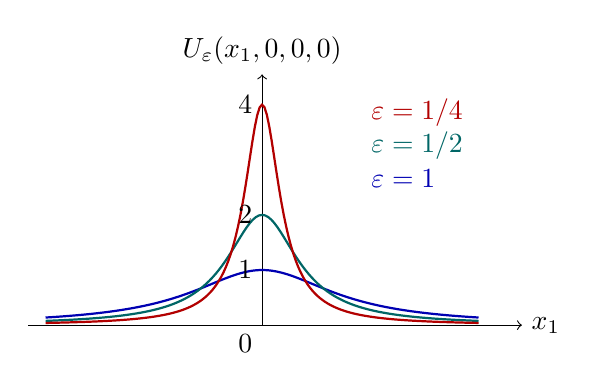
\begin{tikzpicture}[x=1.1cm,y=0.7cm]
	\draw[->] (-2.7,0)--(3.0,0) node[right] {\(x_1\)};
	\draw[->] (0,0)--(0,4.55) node[above] {\(U_\varepsilon(x_1,0,0,0)\)};
	\draw[thick,blue!70!black,domain=-2.5:2.5,samples=141] plot (\x,{1/(1+\x*\x)});
	\draw[thick,teal!80!black,domain=-2.5:2.5,samples=141] plot (\x,{0.5/(0.25+\x*\x)});
	\draw[thick,red!70!black,domain=-2.5:2.5,samples=181] plot (\x,{0.25/(0.0625+\x*\x)});
	\node[left] at (0,1) {\(1\)};
	\node[left] at (0,2) {\(2\)};
	\node[left] at (0,4) {\(4\)};
	\node[blue!70!black,right] at (1.15,2.65) {\(\varepsilon=1\)};
	\node[teal!80!black,right] at (1.15,3.25) {\(\varepsilon=1/2\)};
	\node[red!70!black,right] at (1.15,3.85) {\(\varepsilon=1/4\)};
	\node[below left] at (0,0) {\(0\)};
\end{tikzpicture}

	\caption[临界气泡的尺度变化]{四维时 \(U_\varepsilon(x)=\varepsilon/(\varepsilon^2+|x|^2)\) 的一条径向截面。三条曲线的峰高和宽度不同；保持不变的是四维积分 \(\int_{\mathbb R^4}U_\varepsilon^4\)，而非图中曲线下的平面面积。}
	\label{g3:fig:yamabe-bubbles}
\end{figure}

确定梯度能量的最小代价，需要如下锐形式。它是本节使用的外部分析结果；见\cite[定理3.3，第50页]{LeeParker1987Yamabe}。
\begin{theorem}[锐 Sobolev 不等式]\label{g3:thm:yamabe-sharp-euclidean}
	设 \(n\ge3\)，令
	\[
		Y_S\coloneqq n(n-1)\operatorname{Vol}(S^n,g_{\mathrm{rd}})^{2/n},
	\]
	其中 \(g_{\mathrm{rd}}\) 是截面曲率为一的圆球度量。对每个 \(v\in C_c^\infty(\mathbb R^n)\)，有
	\begin{equation}\label{g3:eq:yamabe-sharp-sobolev}
		Y_S\left(\int_{\mathbb R^n}|v|^p\,\mathrm dx\right)^{2/p}
		\le a_n\int_{\mathbb R^n}|\mathrm Dv|^2\,\mathrm dx.
	\end{equation}
	常数 \(Y_S\) 不能增大。不等式延伸到 \(C_c^\infty\) 关于梯度 \(L^2\) 范数的完备化，在该空间中，式\eqref{g3:eq:yamabe-euclidean-bubble}的函数取得等号。
\end{theorem}
锐常数及气泡等号由所引文献第3节提供。本节从这一精确版本出发，证明它对紧流形极小化序列的后果。完备化中的函数可由式\eqref{g3:eq:yamabe-sharp-sobolev}唯一地解释为 \(L^p\) 函数，因此上述延伸有明确的函数意义。

\begin{proposition}\label{g3:prop:yamabe-sphere-constant}
	对 \(n\ge3\) 的单位圆球，有 \(Y(S^n,[g_{\mathrm{rd}}])=Y_S\)。
\end{proposition}
\begin{proof}
	立体投影把去掉一点的圆球度量写成
	\[
		g_{\mathrm{rd}}=\rho^{4/(n-2)}g_{\mathrm{eucl}},\qquad
		\rho(x)=\left(\frac{2}{1+|x|^2}\right)^{(n-2)/2}.
	\]
	给定光滑 \(w\) 于圆球，记它在这个坐标中的表达仍为 \(w\)，并令 \(F=\rho w\)。\Cref{g3:prop:conformal-laplacian-covariance}的共形能量变换给出
	\[
		\int_{\mathbb R^n}|F|^p\,\mathrm dx
		=\int_{S^n}|w|^p\,\mathrm d\mu_{\mathrm{rd}},
		\qquad
		a_n\int_{\mathbb R^n}|\mathrm DF|^2\,\mathrm dx=E_{g_{\mathrm{rd}}}(w).
	\]
	为核对无穷远处的积分，圆球上的光滑性给出 \(F=O(r^{2-n})\)、\(\mathrm DF=O(r^{1-n})\)。取在 \(B_R\) 上为一、支于 \(B_{2R}\)、梯度不超过 \(C/R\) 的截断 \(\eta_R\)。则 \(\eta_RF\to F\) 于 \(L^p\)，且梯度差的平方积分为 \(O(R^{2-n})\)。因此可以先对紧支函数使用共形公式与分部积分，再令 \(R\to\infty\)；没有留下边界项。

	对 \(\eta_RF\) 应用锐 Sobolev 不等式并取极限，得到 \(Q_{g_{\mathrm{rd}}}(w)\ge Y_S\)。光滑稠密性把它推广到 \(H^1(S^n)\)。另一方面，\(s_{g_{\mathrm{rd}}}=n(n-1)\)，常函数一满足
	\[
		Q_{g_{\mathrm{rd}}}(1)
		=n(n-1)\operatorname{Vol}(S^n,g_{\mathrm{rd}})^{1-2/p}=Y_S.
	\]
	上下界一致。
\end{proof}

现在把气泡放进任意闭流形的一个小坐标球。这个构造同时给出上界与失紧序列，因而解释了为什么必须关注严格不等号。
\begin{proposition}\label{g3:prop:yamabe-bubble-upper-bound}
	设 \((M^n,g)\) 为闭连通光滑黎曼流形，\(n\ge3\)。则 \(Y(M,[g])\le Y_S\)。此外，存在非负 \(v_\varepsilon\in C^\infty(M)\)，满足
	\[
		\|v_\varepsilon\|_p=1,\qquad
		v_\varepsilon\rightharpoonup0\ \text{于 }H^1(M),\qquad
		Q_g(v_\varepsilon)\longrightarrow Y_S.
	\]
	这些函数没有 \(L^p\) 强收敛子列。
\end{proposition}
\begin{proof}
	取一点 \(x_0\) 的正规坐标球 \(B_{2r}(0)\)，以及在 \(B_r\) 上为一、支于 \(B_{2r}\) 的光滑非负截断 \(\chi\)。把 \(b_\varepsilon=\chi U_\varepsilon\) 搬到 \(M\)，在坐标球外补零。换元后，\(g_{ij}(\varepsilon y)\to\delta_{ij}\) 于每个固定球，且原坐标球上的度量与 Euclid 度量一致可比。利用 \(U_1^p\) 和 \(|\mathrm DU_1|^2\) 的可积性，先控制 \(|y|>R\) 的尾部，再令 \(\varepsilon\to0\)、\(R\to\infty\)，得到
	\[
		\int_M b_\varepsilon^p\,\mathrm d\mu_g\longrightarrow
		A\coloneqq\int_{\mathbb R^n}U_1^p\,\mathrm dx>0,
	\qquad
		\int_M|\mathrm db_\varepsilon|^2\,\mathrm d\mu_g
		\longrightarrow\int_{\mathbb R^n}|\mathrm DU_1|^2\,\mathrm dx.
	\]
	第二个极限中的截断误差支于固定环带，在那里 \(U_\varepsilon\) 及其导数均为 \(O(\varepsilon^{(n-2)/2})\)，故误差趋于零。

	零阶项要单独估计。径向积分给出
	\begin{equation}\label{g3:eq:yamabe-bubble-l2}
		\|b_\varepsilon\|_2^2\le C
		\begin{cases}
			\varepsilon,&n=3,\\
			\varepsilon^2\log(1/\varepsilon),&n=4,\\
			\varepsilon^2,&n\ge5,
		\end{cases}
	\end{equation}
	其中取 \(0<\varepsilon<\min\{r,1/2\}\)。例如换元后的积分是常数倍的
	\(\varepsilon^2\int_0^{2r/\varepsilon}t^{n-1}(1+t^2)^{-(n-2)}\,\mathrm dt\)；被积函数在无穷远处为 \(O(t^{3-n})\)，所以出现以上三种情形。由于 \(s_g\) 有界，\(\int s_gb_\varepsilon^2\to0\)。锐不等式在 \(U_1\) 上取等号，遂有 \(Q_g(b_\varepsilon)\to Y_S\)。

	取 \(v_\varepsilon=b_\varepsilon/\|b_\varepsilon\|_p\)。它们在 \(H^1\) 中有界而在 \(L^2\) 中趋于零，因此每个弱收敛子列的极限都为零，故整族弱趋于零。若存在 \(L^p\) 强收敛子列，它也在 \(L^2\) 中趋于同一极限零，与 \(L^p\) 范数恒为一矛盾。最后，由 \(Y(M,[g])\le Q_g(v_\varepsilon)\) 取极限即得上界。
\end{proof}

在任意远离 \(x_0\) 的紧集上，\(v_\varepsilon\) 及其梯度都趋于零；与此同时，\(\int v_\varepsilon^p=1\)。也就是说，体积密度 \(v_\varepsilon^p\,\mathrm d\mu_g\) 的质量集中到 \(x_0\)。这具体说明了临界约束为什么不由弱收敛保留。

\subsection{范数分裂与能量缺陷}
\label{g3:subsec:2404:02}
为处理一般极小化序列，并不需要预先证明它只含一个气泡。只要把弱极限与余项分开，给余项一个带锐常数的能量下界，就足以排除质量丢失。首先把 Euclid 不等式局部化；低阶误差留在 \(L^2\) 项中，而这个范数已有 Rellich 紧性。

\begin{lemma}\label{g3:lem:yamabe-near-sharp-sobolev}
	设 \((M^n,g)\) 为闭光滑黎曼流形，\(n\ge3\)。对每个 \(0<\delta<Y_S\)，存在 \(C_\delta\)，使每个 \(v\in H^1(M)\) 满足
	\begin{equation}\label{g3:eq:yamabe-near-sharp-sobolev}
		(Y_S-\delta)\|v\|_p^2
		\le a_n\|\mathrm dv\|_2^2+C_\delta\|v\|_2^2.
	\end{equation}
\end{lemma}
\begin{proof}
	以充分小的正规坐标球覆盖 \(M\)。度量系数及体积密度与 Euclid 值一致接近，故锐 Euclid 不等式与范数比较说明，对每个支于其中一球的 \(f\)，都有
	\[
		(Y_S-\delta)\|f\|_{L^p(g)}^2\le a_n\|\mathrm df\|_{L^2(g)}^2.
	\]
	这里选球的大小时，将两个比较因子的乘积控制得足够接近一，即可达到给定 \(\delta\)。取从属于有限覆盖的光滑函数 \(\eta_i\)，使 \(\sum_i\eta_i^2=1\)。它们可以从普通单位分解 \(\psi_i\) 构造为 \(\eta_i=\psi_i/(\sum_j\psi_j^2)^{1/2}\)。

	因为 \(p/2>1\)，\(L^{p/2}\) 的三角不等式给出
	\[
		\|v\|_p^2
		=\left\|\sum_i(\eta_iv)^2\right\|_{p/2}
		\le\sum_i\|\eta_iv\|_p^2.
	\]
	局部估计求和后，使用 \(\sum_i\eta_i\,\mathrm d\eta_i=0\)，得到精确恒等式
	\[
		\sum_i|\mathrm d(\eta_iv)|^2
		=|\mathrm dv|^2+v^2\sum_i|\mathrm d\eta_i|^2.
	\]
	最后一项的系数在紧流形上有界，吸收到 \(C_\delta\) 即得结论。先对光滑函数计算，再用 \(H^1\) 光滑稠密性与连续嵌入推广到全部 \(H^1\) 函数。
\end{proof}

下一条范数分裂说明，几乎处处收敛比单纯弱收敛多保留了什么：临界质量虽可能丢失，却可以准确归入余项。
\begin{lemma}\label{g3:lem:yamabe-norm-splitting}
	设 \((X,\mu)\) 为测度空间，\(1<q<\infty\)。若实函数列 \(f_j\) 在 \(L^q(X)\) 中有界，且几乎处处趋于 \(f\)，则 \(f\in L^q(X)\)，并有
	\begin{equation}\label{g3:eq:yamabe-norm-splitting}
		\int_X|f_j|^q\,\mathrm d\mu
		=\int_X|f|^q\,\mathrm d\mu
		+\int_X|f_j-f|^q\,\mathrm d\mu+o(1).
	\end{equation}
\end{lemma}
\begin{proof}
	Fatou 引理给出 \(f\in L^q\)，故 \(h_j=f_j-f\) 也在 \(L^q\) 中有界。对每个 \(\epsilon>0\)，中值公式和 Young 不等式给出
	\[
		\bigl||a+b|^q-|a|^q\bigr|
		\le\epsilon|a|^q+C_\epsilon|b|^q,
		\qquad a,b\in\mathbb R.
	\]
	具体地，中值公式先给出 \(C_q(|a|^{q-1}|b|+|b|^q)\)，再用共轭指数 \(q/(q-1)\) 与 \(q\) 即得所示形式。令
	\[
		d_j=|f_j|^q-|h_j|^q-|f|^q,
		\qquad r_j=(|d_j|-\epsilon|h_j|^q)_+.
	\]
	由于 \(h_j\to0\) 几乎处处，有 \(r_j\to0\) 几乎处处；上式又给 \(0\le r_j\le(C_\epsilon+1)|f|^q\)。支配收敛定理于是给出 \(\int r_j\to0\)。因此
	\[
		\limsup_j\int_X|d_j|\,\mathrm d\mu
		\le\epsilon\sup_j\|h_j\|_q^q.
	\]
	令 \(\epsilon\downarrow0\) 即得 \(d_j\to0\) 于 \(L^1\)，从而得到所需等式。
\end{proof}

\begin{lemma}\label{g3:lem:yamabe-energy-defect}
	设 \((M^n,g)\) 为闭光滑黎曼流形，\(n\ge3\)。设实函数 \(u_j\rightharpoonup u\) 于 \(H^1(M)\)，\(\|u_j\|_p=1\)，且 \(E_g(u_j)\to\ell\)。则
	\begin{equation}\label{g3:eq:yamabe-energy-defect}
		\ell\ge E_g(u)+Y_S(1-\|u\|_p^p)^{2/p}.
	\end{equation}
\end{lemma}
\begin{proof}
	由\cref{g3:thm:compact-bundle-rellich}，弱收敛列在 \(L^2\) 中强趋于 \(u\)；取子列后也几乎处处收敛。写 \(w_j=u_j-u\)。前一引理给出
	\[
		\|w_j\|_p^p\longrightarrow1-\|u\|_p^p\ge0.
	\]
	弱收敛使梯度交叉项趋于零，\(L^2\) 强收敛使所有含 \(s_g\) 的余项趋于零。因此
	\[
		E_g(u_j)=E_g(u)+a_n\|\mathrm dw_j\|_2^2+o(1).
	\]
	对 \(w_j\) 使用式\eqref{g3:eq:yamabe-near-sharp-sobolev}，先令 \(j\to\infty\)；因为 \(\|w_j\|_2\to0\)，得到
	\[
		\ell-E_g(u)\ge(Y_S-\delta)(1-\|u\|_p^p)^{2/p}.
	\]
	再令 \(\delta\downarrow0\)，得到结论。各个子列产生同一个不等式，所以取几乎处处收敛子列不影响断言。
\end{proof}

这就是本章所需的\term[jizhong jin xing]{集中紧性}[concentration compactness]估计：余项携带的临界质量为 \(1-\|u\|_p^p\)，它的能量至少为这份质量的 \(2/p\) 次幂乘以 \(Y_S\)。证明没有预设余项的空间形状，因而也涵盖多个区域中的集中。

\subsection{低于球面常数时排除集中}
\label{g3:subsec:2404:03}
记 \(Y=Y(M,[g])\)，并令 \(\alpha=2/p=(n-2)/n\in(0,1)\)。若 \(\|u_j\|_p=1\)、\(E_g(u_j)\to Y\)，能量缺陷估计与 \(E_g(u)\ge Y\|u\|_p^2\) 将给出
\begin{equation}\label{g3:eq:yamabe-mass-comparison}
	Y\ge Yt^\alpha+Y_S(1-t)^\alpha,
	\qquad t=\|u\|_p^p\in[0,1].
\end{equation}
这里 \(t=0\) 表示所有临界质量都离开弱极限，\(0<t<1\) 表示只保住一部分，\(t=1\) 表示没有丢失。下面的代数比较同时处理这三种可能。

\begin{lemma}\label{g3:lem:yamabe-threshold-exclusion}
	设 \(Y<Y_S\)、\(Y_S>0\)、\(0<\alpha<1\)。若 \(t\in[0,1]\) 满足式\eqref{g3:eq:yamabe-mass-comparison}，则 \(t=1\)。
\end{lemma}
\begin{proof}
	若 \(t=0\)，式子给出 \(Y\ge Y_S\)，矛盾。若 \(0<t<1\) 且 \(Y>0\)，则
	\[
		Yt^\alpha+Y_S(1-t)^\alpha
		>Y\bigl(t^\alpha+(1-t)^\alpha\bigr)>Y,
	\]
	因为 \(t^\alpha>t\)、\((1-t)^\alpha>1-t\)。若 \(Y\le0\)，则
	\[
		Yt^\alpha+Y_S(1-t)^\alpha-Y
		=Y(t^\alpha-1)+Y_S(1-t)^\alpha>0;
	\]
	第一项非负，第二项为正。这同样与假设矛盾。只剩 \(t=1\)。
\end{proof}

严格阈值有两个作用。全部集中时，代价 \(Y_S\) 已经高于极小值 \(Y\)；部分集中时，指数 \(\alpha<1\) 又使质量拆分增加代价。这解释了为何不必先定位集中点，也能证明极小化序列紧。

\subsection{严格阈值下的极小值实现}
\label{g3:subsec:2404:04}
\begin{theorem}\label{g3:thm:yamabe-below-sphere}
	设 \((M^n,g)\) 为闭连通光滑黎曼流形，\(n\ge3\)，且
	\[
		Y(M,[g])<Y(S^n,[g_{\mathrm{rd}}])=Y_S.
	\]
	则存在光滑正函数 \(u\)，使 \(\int_Mu^p\,\mathrm d\mu_g=1\)、\(E_g(u)=Y(M,[g])\)。它满足
	\[
		L_gu=Y(M,[g])u^{p-1},
	\]
	度量 \(u^{4/(n-2)}g\) 具有体积一和常标量曲率 \(Y(M,[g])\)。每个归一化的非负极小化序列，都有在 \(H^1(M)\) 中强收敛到某个这样的极小函数的子列。
\end{theorem}
\begin{proof}
	记 \(Y=Y(M,[g])\)，取非负极小化序列 \(u_j\)，满足 \(\|u_j\|_p=1\)。Hölder 不等式给出 \(\|u_j\|_2^2\le\operatorname{Vol}(M,g)^{2/n}\)，而
	\[
		a_n\|\mathrm du_j\|_2^2
		\le E_g(u_j)+\|s_g^-\|_\infty\|u_j\|_2^2,
		\qquad s_g^-=\max\{-s_g,0\}.
	\]
	故 \(u_j\) 在 \(H^1\) 中有界。取弱收敛子列 \(u_j\rightharpoonup u\)，由 Rellich 紧性进一步取 \(L^2\) 及几乎处处收敛子列。因此 \(u\ge0\)，且 \(t=\|u\|_p^p\le1\)。

	由能量缺陷估计以及 Yamabe 常数的定义，得到式\eqref{g3:eq:yamabe-mass-comparison}；当 \(u=0\) 时，\(E_g(u)\ge Y\|u\|_p^2\) 也成立。\Cref{g3:lem:yamabe-threshold-exclusion}给出 \(t=1\)。于是 \(u\) 保留全部约束，且
	\[
		Y\le E_g(u)\le\liminf_jE_g(u_j)=Y.
	\]
	这里第二个不等式使用梯度范数弱下半连续性与势能项的 \(L^2\) 连续性。所以 \(u\) 取得极小值。

	还有强收敛。由 \(E_g(u_j)\to E_g(u)\) 及 \(L^2\) 强收敛，得到 \(\|\mathrm du_j\|_2\to\|\mathrm du\|_2\)。Hilbert 空间中的弱收敛与范数收敛推出梯度强收敛，结合 \(L^2\) 收敛即得 \(H^1\) 强收敛。连续 Sobolev 嵌入同时给出 \(L^p\) 强收敛。

	\Cref{g3:prop:yamabe-euler-lagrange}的约束变分给出所示弱方程，\(u\not\equiv0\)。\Cref{g3:thm:yamabe-weak-regularity}把它提升为光滑正解；共形标量曲率及体积公式给出度量的结论。对任意归一化非负极小化序列，上述步骤都适用，故也得到最后的紧性断言。
\end{proof}

\begin{example}\label{g3:exm:yamabe-threshold-sharpness}
	在圆球上，\(Y=Y_S\)，极小值已由常函数取得；但\cref{g3:prop:yamabe-bubble-upper-bound}给出的截断气泡仍是归一化极小化序列，并且弱趋于零。因此，极小值存在不意味着所有极小化序列紧。严格阈值定理同时证明存在性与序列紧性，而等号情形至少需要另行处理其中的集中行为。
\end{example}

至此，剩余问题集中为一个几何比较：除圆球共形类之外，如何把某个测试函数的商压到 \(Y_S\) 以下？普通坐标中的截断气泡只给极限上界；严格改进要使用曲率展开或 Green 函数的整体信息。
% 纲要条目排为编号小节标题，并进入目录与书签；说明段仍保留于纲要注释中。

% !TeX root = ../../Book3.tex
% 纲要标题：### 24.5 Yamabe 问题的一般存在性
% 纲要位置：几何学计划纲要.md，第 3156 行。
% 正文状态：初稿，尚未正式审核。

% 纲要内容开始
% 
% * Aubin 型测试函数
% * 低维与局部共形平坦情形
% * 正质量定理与 Schoen 方法
% * 局部极小、全局极小和非唯一解
% 
% ---
% 
% 纲要内容结束

\section{Yamabe 问题的一般存在性}
\label{g3:sec:2405}

严格阈值定理把一般存在性归结为一个具体问题：当共形类不是圆球面的共形类时，怎样找出一个满足 \(Q_g(v)<Y_S\) 的测试函数？截断气泡只给出趋近球面常数的函数列。要使商严格下降，还须读出气泡所处几何对能量的下一阶贡献。局部曲率足以处理一部分情形，剩下的情形则需要把测试函数延伸到整个流形。

\subsection{Aubin 型测试函数}
\label{g3:subsec:2405:01}
第3章的\cref{g3:prop:conformal-weyl}说明，四阶协变 Weyl 张量在 \(\widehat g=e^{2f}g\) 下变为 \(e^{2f}W_g\)。因此 \(W_g(q)\ne0\) 不能靠改变共形代表消去。Aubin 的测试函数利用这一点：先选择共形代表，使法坐标中的低阶体积误差尽量消失，再把径向气泡放在 \(W_g\ne0\) 的点附近。下面所引定理包括这一共形规范的构造和曲率项的符号计算。

\begin{theorem}[Aubin 的严格不等式]\label{g3:thm:yamabe-aubin-strict}
	记 \(Y_S=n(n-1)\operatorname{Vol}(S^n,g_{\mathrm{rd}})^{2/n}\)，\(g_{\mathrm{rd}}\) 为曲率一的圆球度量。
	设 \((M^n,g)\) 是闭连通光滑黎曼流形，\(n\ge6\)。若 \((M,g)\) 不是局部共形平坦的，则
	\[
		Y(M,[g])<Y_S.
	\]
	这里局部共形平坦是指每点都有邻域，在该邻域内 \(g\) 是某个 Euclid 度量的正光滑函数倍数。
\end{theorem}
这一结果及其与 Weyl 张量的关系见\cite[定理B，第39页；第5、11节]{LeeParker1987Yamabe}。所用的局部共形平坦判别是 \(n\ge4\) 时 \(W\equiv0\) 当且仅当局部共形平坦；本卷第3章已经证明其中由局部共形平坦推出 \(W=0\) 的方向，反方向及测试函数的高阶规范在这里随外部结果调用。

\ProseParagraphBreak
维数 \(6\) 的分界可以从一个径向积分看出。取
\[
	U_\varepsilon(r)=\left(\frac{\varepsilon}{\varepsilon^2+r^2}\right)^{(n-2)/2},
	\qquad 0<\varepsilon<\rho,
\]
其中 \(\rho\) 固定。记 \(\sigma_{n-1}=\operatorname{Vol}(S^{n-1})\)。计算局部曲率修正时会遇到
\begin{equation}\label{g3:eq:yamabe-curvature-moment}
	\int_{B_\rho}|x|^2U_\varepsilon^2\,\mathrm dx
	=\sigma_{n-1}\varepsilon^4
	\int_0^{\rho/\varepsilon}\frac{t^{n+1}}{(1+t^2)^{n-2}}\,\mathrm dt.
\end{equation}
等式由极坐标和 \(r=\varepsilon t\) 直接得到。被积函数在无穷远与 \(t^{5-n}\) 同阶，所以 \(n\ge7\) 时右侧与 \(\varepsilon^4\) 同阶，\(n=6\) 时则与 \(\varepsilon^4\log(1/\varepsilon)\) 同阶。另一方面，固定环带内截断气泡的梯度误差是 \(O(\varepsilon^{n-2})\)。前两种曲率修正都能支配截断误差；外引定理的关键计算进一步说明，经过共形规范后，非零 Weyl 曲率贡献所需的下降方向。尺度比较解释了这个计算为何可能成功，下降的符号则来自完整的曲率展开。

\subsection{低维与局部共形平坦情形}
\label{g3:subsec:2405:02}
对 \(n=3,4,5\)，式\eqref{g3:eq:yamabe-curvature-moment}分别与 \(\varepsilon\)、\(\varepsilon^2\)、\(\varepsilon^3\) 同阶，恰与 \(\varepsilon^{n-2}\) 的截断误差处于同一尺度。缩小气泡便不能单凭阶数把误差压到主项以下。在局部共形平坦情形，困难更直接：可以选取在一个小球内完全平坦的共形代表，这时只支于该球内的测试函数受到 Euclid 最佳 Sobolev 不等式的约束。

\begin{proposition}\label{g3:prop:yamabe-flat-local-tests}
	对所用度量 \(h\)，记 \(E_h(v)=\int_M(\tfrac{4(n-1)}{n-2}|\mathrm dv|_h^2+s_hv^2)\,\mathrm d\mu_h\)，\(Q_h(v)=E_h(v)/\|v\|_{L^{2n/(n-2)}(h)}^2\)（\(v\ne0\)）。记 \(Y_S=n(n-1)\operatorname{Vol}(S^n,g_{\mathrm{rd}})^{2/n}\)，\(g_{\mathrm{rd}}\) 为曲率一的圆球度量。
	设 \((M^n,g)\) 为光滑黎曼流形，\(n\ge3\)，且某开集 \(V\) 在坐标下的度量恰为 Euclid 度量。对每个非零 \(v\in C_c^\infty(V)\)，有
	\[
		Q_g(v)\ge Y_S.
	\]
	若在同一个坐标开集 \(V\) 上有 \(g=\phi^{4/(n-2)}g_{\mathrm E}\)、\(\phi>0\) 光滑，同一结论仍适用于支于 \(V\) 的测试函数。
\end{proposition}
\begin{proof}
	平坦情形下 \(s_g=0\)，把 \(v\) 经坐标送到 Euclid 空间并补零，\cref{g3:thm:yamabe-sharp-euclidean}给出
	\[
		Q_g(v)=\frac{a_n\int_{\mathbb R^n}|\mathrm dv|^2\,\mathrm dx}
		{(\int_{\mathbb R^n}|v|^p\,\mathrm dx)^{2/p}}
		\ge Y_S.
	\]
	一般情形写 \(g=\phi^{4/(n-2)}g_0\)，其中 \(g_0\) 在 \(V\) 上平坦，\(\phi>0\)。由\cref{g3:prop:conformal-laplacian-covariance}，对支于 \(V\) 的函数有 \(Q_g(v)=Q_{g_0}(\phi v)\)。函数 \(\phi v\) 仍紧支于 \(V\)，故归结为第一种情形。
\end{proof}
这解释了为何局部共形平坦流形的严格不等式必须看到小球之外的几何。球面空间形式在小邻域内与圆球面没有共形区别，整体的覆盖结构却能使 Yamabe 常数严格下降。

\begin{example}\label{g3:exm:yamabe-spherical-quotient}
	设 \(n\ge3\)，有限群 \(\Gamma\) 在曲率为一的圆球面 \((S^n,g_{\mathrm{rd}})\) 上自由、等距地作用。令 \(d=|\Gamma|\)，\(M=S^n/\Gamma\)，\(g\) 为诱导商度量，\(\pi:S^n\to M\) 为覆盖映射。记
	\[
		p=\frac{2n}{n-2},\qquad a_n=\frac{4(n-1)}{n-2},
		\qquad Y_S=n(n-1)\operatorname{Vol}(S^n,g_{\mathrm{rd}})^{2/n}.
	\]
	对所用度量 \(h\)，令
	\[
		E_h(v)=\int\bigl(a_n|\mathrm dv|_h^2+s_hv^2\bigr)\,\mathrm d\mu_h,
		\qquad Q_h(v)=\frac{E_h(v)}{\|v\|_{L^p(h)}^2}\quad(v\ne0).
	\]
	则商流形的 Yamabe 常数为
	\[
		Y(M,[g])=d^{-2/n}Y_S.
	\]
	为证明下界，取任意非零 \(u\in H^1(M)\)。覆盖映射是局部等距，每点有 \(d\) 个原像，所以按覆盖片积分得到
	\[
		E_{g_{\mathrm{rd}}}(u\circ\pi)=dE_g(u),
		\qquad
		\|u\circ\pi\|_{L^p(g_{\mathrm{rd}})}^2
		=d^{2/p}\|u\|_{L^p(g)}^2.
	\]
	这些公式可先对光滑函数验证，再由光滑函数在 \(H^1\) 中稠密及 Sobolev 嵌入推广到上述 \(u\)。因此
	\[
		Q_{g_{\mathrm{rd}}}(u\circ\pi)=d^{1-2/p}Q_g(u)
		=d^{2/n}Q_g(u).
	\]
	由\cref{g3:prop:yamabe-sphere-constant}，左侧至少为 \(Y_S\)，故对全部竞争函数都有 \(Q_g(u)\ge d^{-2/n}Y_S\)。另一方面，局部等距性给出 \(s_g=n(n-1)\)，且 \(\operatorname{Vol}_g(M)=\operatorname{Vol}(S^n,g_{\mathrm{rd}})/d\)，从而
	\[
		Q_g(1)=n(n-1)\bigl(\operatorname{Vol}(S^n,g_{\mathrm{rd}})/d\bigr)^{2/n}
		=d^{-2/n}Y_S.
	\]
	上下界一致，且常数函数实现极小值。若 \(d>1\)，所得常数严格小于 \(Y_S\)。商流形局部共形平坦，\cref{g3:prop:yamabe-flat-local-tests}却保证每个紧支于一个共形平坦坐标小球的非零测试函数仍满足 \(Q_g(v)\ge Y_S\)。所以这里的下降由遍及商流形的测试函数反映，不能只从一个小球内的几何得到。
\end{example}

\ProseParagraphBreak
延伸测试函数时，希望其在气泡之外的能量尽可能小。那里函数的值很小，方程中的 \(u^{p-1}\) 比 \(u\) 衰减更快，因此先求线性方程 \(L_gu=0\) 是自然的选择。带一个极点的正 Green 函数正好同时满足这个方程，并具有与气泡远场相匹配的 \(r^{2-n}\) 奇性。

\subsection{正质量定理与 Schoen 方法}
\label{g3:subsec:2405:03}
设 \(Y(M,[g])>0\)。固定 \(q\in M\)，将共形 Laplace 的 Green 函数归一化为
\begin{equation}\label{g3:eq:yamabe-green-normalization}
	L_gG_q=a_n(n-2)\sigma_{n-1}\delta_q,
	\qquad G_q(x)\sim d_g(x,q)^{2-n}.
\end{equation}
这里 Dirac 分布以 \(g\) 的体积密度解释。正性条件使 \(L_g\) 可逆；Green 函数的存在、严格正性及所需局部展开见\cite[引理6.1、6.4，定理6.5]{LeeParker1987Yamabe}。先看 \(g\) 在 \(q\) 附近平坦的情形，此时
\[
	G_q(x)=|x|^{2-n}+A_q+O(|x|).
\]
减去基本解后留下的是光滑调和函数，所以这里的余项也可逐次微分。定义穿孔流形上的度量
\begin{equation}\label{g3:eq:yamabe-green-blowup}
	g_\infty=G_q^{4/(n-2)}g
	\quad\text{于 }M\setminus\{q\}.
\end{equation}
由标量曲率变换公式，\(s_{g_\infty}=0\)。在 \(q\) 附近，径向长度与 \(r^{-2}\,\mathrm dr\) 可比，到 \(q\) 的距离无穷大；其余部分来自紧流形。故 \(g_\infty\) 完备，原来的点变成一个无穷远端。

\ProseParagraphBreak
作反演 \(y=x/|x|^2\)，记 \(R=|y|\)。Euclid 度量在反演下贡献 \(R^{-4}\)，它与 Green 函数主项的共形倍数抵消，得到
\begin{equation}\label{g3:eq:yamabe-green-af}
	(g_\infty)_{ij}(y)
	=\bigl(1+A_qR^{2-n}+O(R^{1-n})\bigr)^{4/(n-2)}\delta_{ij}.
\end{equation}
这类在无穷远趋于 Euclid 度量，并且一、二阶导数有相应衰减的度量称为\term[jianjinpingtanduoliang]{渐近平坦度量}[asymptotically flat metric]。在坐标满足
\(h_{ij}-\delta_{ij}=O(R^{-\tau})\)、其一、二阶导数分别为 \(O(R^{-\tau-1})\)、\(O(R^{-\tau-2})\)，其中 \(\tau>(n-2)/2\)，且标量曲率可积时，所用质量归一化为
\begin{equation}\label{g3:eq:yamabe-adm-mass}
	m(h)=\frac1{2(n-1)\sigma_{n-1}}
	\lim_{R\to\infty}\int_{|y|=R}
	\sum_{i,j}(\partial_jh_{ij}-\partial_ih_{jj})\nu^i\,\mathrm dS.
\end{equation}
法向和面积元在此按 Euclid 度量计算。在这组衰减与可积条件下，极限的存在及坐标不变性可由\cite[第9节，定理9.6]{LeeParker1987Yamabe}核对；该文的质量比式\eqref{g3:eq:yamabe-adm-mass}大 \(2(n-1)\) 倍。对式\eqref{g3:eq:yamabe-green-af}，令括号的 \(4/(n-2)\) 次幂为 \(f\)，便有
\[
	\sum_j(\partial_jh_{ij}-\partial_ih_{jj})
	=-(n-1)\partial_if,
	\qquad
	\partial_R f=-4A_qR^{1-n}+O(R^{-n}),
\]
从而直接算得
\begin{equation}\label{g3:eq:yamabe-mass-green-coefficient}
	m(g_\infty)=2A_q.
\end{equation}
Green 函数的常数项因此记录了整个穿孔流形的几何，而不只是极点处有限阶的曲率。

\begin{theorem}\label{g3:thm:yamabe-green-positive-mass}
	设 \((M^n,g)\) 为闭连通光滑黎曼流形，\(n\ge3\)、\(Y(M,[g])>0\)，并满足以下条件之一：\(3\le n\le5\)；或 \((M,g)\) 局部共形平坦。任取 \(q\in M\)，在 \(q\) 附近先选择共形法坐标代表，局部共形平坦时可选为平坦代表，再按式\eqref{g3:eq:yamabe-green-normalization}归一化 Green 函数。令 \(g_\infty=G_q^{4/(n-2)}g\)，其中 \(G_q\) 是所选代表的上述归一化 Green 函数，\(m\) 为式\eqref{g3:eq:yamabe-adm-mass}的渐近平坦质量。则 \((M\setminus\{q\},g_\infty)\) 是完备、标量曲率为零的渐近平坦流形，其质量满足
	\[
		m(g_\infty)\ge0.
	\]
	质量为零当且仅当 \((M,[g])\) 与标准圆球面的共形类共形微分同胚；此时吹起度量等距于 Euclid 空间。
\end{theorem}
这里的共形法坐标可使体积密度在任意预先指定的有限阶上等于 Euclid 密度。低维时这一步保证渐近衰减足够快，并把质量与 Green 函数的常数项联系起来。对应的展开、质量联系与零质量刚性见\cite[引理6.4、9.7，第10节]{LeeParker1987Yamabe}及\cite[第2节，引理3、命题2]{Schoen1984Yamabe}。局部共形平坦的高维情形使用闭流形 Green 函数的特殊正质量结论，见\cite[命题3.3(i)、4.4，第62、65页]{SchoenYau1988ConformallyFlat}：先以第一特征函数选取正标量曲率代表，其覆盖空间上的标量曲率有正下界，四维所需的 Ricci 有界性也由紧性得到。这个版本只涉及上述 Green 函数吹起，不增加一般高维渐近平坦流形的假设范围。

\ProseParagraphBreak
若原流形不共形于球面，质量的严格正性提供了局部气泡没有的下降量。Schoen 把气泡的核心与小倍数 \(G_q\) 的远场接合，在环带中匹配两者。局部平坦时，分部积分把远场能量化为球面边界项，\(A_q>0\) 使关键边界项为负；先把接合半径取得足够小，再缩小气泡尺度，就能使接合误差小于这个负项。三维的一般 Green 展开仍能支持同样的构造；四、五维还需控制度量不平坦所产生的误差。精确的存在结论如下。

\begin{theorem}[Schoen 的严格不等式]\label{g3:thm:yamabe-schoen-strict}
	记 \(Y_S=n(n-1)\operatorname{Vol}(S^n,g_{\mathrm{rd}})^{2/n}\)，\(g_{\mathrm{rd}}\) 为曲率一的圆球度量。
	设 \((M^n,g)\) 为闭连通光滑黎曼流形，\(n\ge3\)。若 \(3\le n\le5\)，或 \((M,g)\) 局部共形平坦，并且 \((M,[g])\) 不共形微分同胚于标准圆球面的共形类，则
	\[
		Y(M,[g])<Y_S.
	\]
\end{theorem}
局部平坦附近的接合及三维情形见\cite[第1节，定理1、命题1，第481--484页]{Schoen1984Yamabe}；低维剩余估计及严格不等式见该文第2节、定理2（第493页）。其中作者把泛函除以了本章的 \(a_n\)，这个正因子不改变严格不等式。上述测试函数估计和正质量定理是本节外引的深层内容；下面的存在性结论只需把它们与已经证明的紧性相接。

\begin{corollary}[Yamabe 问题的一般存在性]\label{g3:cor:yamabe-general-existence}
	记 \(p=2n/(n-2)\)。共形 Laplace 算子取 \(L_g=\tfrac{4(n-1)}{n-2}\Delta_g+s_g\)，其中 \(\Delta_g=-\operatorname{div}_g\nabla\)。
	每个闭连通光滑黎曼流形 \((M^n,g)\)、\(n\ge3\)，都存在 \(u\in C^\infty(M)\)、\(u>0\)，使
	\[
		\int_Mu^p\,\mu_g=1,
		\qquad L_gu=Y(M,[g])u^{p-1}.
	\]
	因此 \(u^{4/(n-2)}g\) 是该共形类内体积为一、标量曲率恒等于 \(Y(M,[g])\) 的度量。
\end{corollary}
\begin{proof}
	若 \((M,[g])\) 是圆球面的共形类，取圆度量的拉回并作常数缩放，体积归一后即得结论。否则，在 \(n\ge6\) 且非局部共形平坦时应用\cref{g3:thm:yamabe-aubin-strict}，其余情形应用\cref{g3:thm:yamabe-schoen-strict}，均有 \(Y(M,[g])<Y_S\)。由\cref{g3:thm:yamabe-below-sphere}，存在归一化非负极小函数；\cref{g3:thm:yamabe-weak-regularity}将它提升为光滑正解。标量曲率与体积公式给出最后结论。
\end{proof}

\subsection{局部极小、全局极小和非唯一解}
\label{g3:subsec:2405:04}
上述存在性得到的是 Yamabe 泛函的全局极小值。一个任意的常标量曲率度量只保证泛函一阶变分为零，其二阶行为还要另行判断。为了把二阶条件写成普通 Laplace 谱，直接把待考察的常标量曲率度量作为背景度量。

\begin{proposition}\label{g3:prop:yamabe-csc-stability}
	记 \(p=2n/(n-2)\)。对所用度量 \(h\)，记 \(E_h(v)=\int_M(\tfrac{4(n-1)}{n-2}|\mathrm dv|_h^2+s_hv^2)\,\mathrm d\mu_h\)，\(Q_h(v)=E_h(v)/\|v\|_{L^{2n/(n-2)}(h)}^2\)（\(v\ne0\)）。
	设 \((M^n,g)\) 为闭连通光滑黎曼流形，\(n\ge3\)，\(\operatorname{Vol}_g(M)=1\)，且 \(s_g=s\) 为常数。令 \(\lambda_1(\Delta_g)\) 为标量 Laplace 的第一正特征值。函数 \(1\) 是约束 \(\int_M|v|^p\,\mu_g=1\) 上 \(E_g\) 的临界点，并有以下结论。
	\begin{enumerate}
		\item 若 \(1\) 是局部极小点，则 \(\lambda_1(\Delta_g)\ge s/(n-1)\)。
		\item 若 \(\lambda_1(\Delta_g)>s/(n-1)\)，则 \(1\) 是该约束集上相对于 \(H^1\) 拓扑的严格局部极小点。
		\item 若 \(\lambda_1(\Delta_g)<s/(n-1)\)，则存在保持体积的光滑正共形变化，使泛函在 \(g\) 附近严格下降。
	\end{enumerate}
\end{proposition}
\begin{proof}
	体积约束的切空间是 \(\int_Mh\,\mu_g=0\)。把 \(u=1\)、\(\lambda=s\) 代入\cref{g3:prop:yamabe-second-variation}，约束 Hessian 为
	\begin{equation}\label{g3:eq:yamabe-csc-hessian}
		2a_n\left(\int_M|\mathrm dh|^2\,\mu_g
		-\frac{s}{n-1}\int_Mh^2\,\mu_g\right),
	\end{equation}
	因为 \((p-2)/a_n=1/(n-1)\)。式\eqref{g3:eq:first-eigenvalue-mean-zero}正是平均值为零函数的 Rayleigh 商表述，故局部极小时 Hessian 非负给出第一项。若出现严格反向不等式，取第一特征函数 \(h\)，沿
	\[
		v_t=\frac{1+th}{\|1+th\|_p}
	\]
	变化。\(h\) 光滑有界，所以 \(|t|\) 足够小时 \(v_t>0\)；一阶导数为零而二阶导数为负，得到第三项。

	设谱隙为严格正。Poincar\'e 不等式使式\eqref{g3:eq:yamabe-csc-hessian}在平均值为零的子空间上至少为 \(c\|h\|_{H^1}^2\)，其中 \(c>0\)。映射 \(v\mapsto\int_M|v|^p\,\mu_g\) 在 \(H^1\) 上为 \(C^2\)，且在 \(1\) 处的导数是 \(h\mapsto p\int_Mh\,\mu_g\)，在常数方向可逆。\cref{g3:cor:banach-implicit-parameters}因此把约束集在 \(1\) 附近写成平均值为零子空间上的 \(C^2\) 图。把 \(E_g\) 限制到这个图，Taylor 公式给出
	\[
		E_g(v)-E_g(1)\ge\frac c4\|h\|_{H^1}^2>0
	\]
	对足够小的非零参数 \(h\) 成立，证明第二项。
\end{proof}
等号 \(\lambda_1=s/(n-1)\) 只说明存在二阶零方向。它可能来自共形对称，判断局部极小还需使用高阶信息或已知的全局极小性质。另一方面，严格局部极小控制的是一个邻域；全局极小还须比较远离该邻域的共形因子。

\begin{example}\label{g3:exm:yamabe-sphere-nonuniqueness}
	记 \(Y_S=n(n-1)\operatorname{Vol}(S^n,g_{\mathrm{rd}})^{2/n}\)，其中 \(g_{\mathrm{rd}}\) 为曲率一的圆球度量。
	设 \(n\ge3\)，令 \(\bar g\) 是体积为一的圆球面度量。以立体投影坐标 \(x\in\mathbb R^n\) 表示球面去掉一点，Euclid 伸缩 \(x\mapsto tx\)、\(t>0\)，延伸为球面的共形微分同胚 \(F_t\)，且
	\[
		F_t^*\bar g=v_t^{4/(n-2)}\bar g,
		\qquad
		v_t(x)=\left(\frac{t(1+|x|^2)}{1+t^2|x|^2}\right)^{(n-2)/2}.
	\]
	在被删去的点使用反演坐标，上式仍为光滑正函数。由于拉回保持总体积和标量曲率，\(\|v_t\|_p=1\)、\(Q_{\bar g}(v_t)=Y_S\)。\(t\ne1\) 时 \(v_t\) 非常数，故同一个正 Yamabe 共形类内，体积为一的极小函数和作为固定流形上张量的极小度量都不唯一。这些度量彼此等距；若再模去共形微分同胚，它们属于同一类。
\end{example}

\begin{example}\label{g3:exm:yamabe-long-cylinder}
	设 \(n\ge3\)、\(L>0\)。在 \(S_L^1\times S^{n-1}\) 上取乘积度量，圆周长度为 \(L\)，球面半径为一。其标量曲率为 \((n-1)(n-2)\)。函数 \(h(t,\theta)=\cos(2\pi t/L)\) 的平均值为零，Rayleigh 商为 \((2\pi/L)^2\)。若
	\[
		L>\frac{2\pi}{\sqrt{n-2}},
	\]
	式\eqref{g3:eq:yamabe-csc-hessian}在这个方向为负。把度量缩放到体积一时，标量曲率和 Laplace 特征值乘以相同因子，负号保持不变。因此该乘积度量虽是常标量曲率度量，却不是所在共形类的局部极小度量。一般存在性推论保证该共形类另有一个全局极小度量。
\end{example}
正情形的三个问题由此分开：Euler--Lagrange 方程决定临界点，约束 Hessian 检验局部稳定性，而严格球面阈值和极小化序列的紧性给出全局极小值。体积约束只消去常数缩放，不能消去球面的非平凡共形对称。
% 纲要条目排为编号小节标题，并进入目录与书签；说明段仍保留于纲要注释中。


\begin{chaptersummary}
	在 \(n\ge3\) 维，共形变化 \(g_u=u^{4/(n-2)}g\) 使体积变为 \(u^p\mu_g\)，标量曲率变为 \(u^{1-p}L_gu\)，其中 \(p=2n/(n-2)\)、\(L_g=4(n-1)\Delta_g/(n-2)+s_g\)。共形能量满足 \(E_{g_u}(v)=E_g(uv)\)，所以 Yamabe 常数只依赖指定共形类。体积约束产生的乘子就是极小度量的常标量曲率。

	\ProseParagraphBreak
	非负弱解首先属于临界 Sobolev 空间。将方程写成 \(\Delta_gu=Vu\)，截断测试和 \(L^{n/2}\) 尾部吸收提高其可积指数，继而椭圆估计、强最大值原理和光滑复合给出光滑正解。最低特征值与 Yamabe 常数同号；线性核、常数缩放和非线性唯一性分别由不同条件决定。

	\ProseParagraphBreak
	当 \(Y\le0\) 时，归一化极小化序列的弱极限非零，能量等号恢复强 \(H^1\) 收敛。所得单位体积常标量曲率度量在共形类中唯一。正情形需要球面阈值：临界气泡保持梯度能量和 \(L^p\) 质量，近锐 Sobolev 估计则把丢失的质量换成至少为球面常数所决定的能量代价。范数分裂与极小性共同排除全部或部分集中，从而证明 \(Y<Y_S\) 时的极小值实现和极小化序列紧性。

	\ProseParagraphBreak
	一般存在性还需要严格阈值的几何来源。非局部共形平坦的高维情形使用 Weyl 曲率对气泡能量的修正，低维或局部共形平坦情形使用 Green 函数吹起与正质量。准确调用这些结果后，除圆球共形类外均落入严格阈值；圆球自身有显式极小度量。正情形的解可以不唯一，常标量曲率度量也可以不是局部极小点，约束 Hessian 和明确的共形模型分别揭示这两种现象。
\end{chaptersummary}

\BookExercises

\begin{exercise}\label{g3:ex:yamabe-background-scaling}
	设 \(c>0\)，令 \(h=c^2g\)。证明
	\[
		L_h=c^{-2}L_g,\quad E_h(u)=c^{n-2}E_g(u),\quad
		\|u\|_{L^p(h)}^2=c^{n-2}\|u\|_{L^p(g)}^2.
	\]
	求 \(Y(M,[h])\) 与 \(\lambda_1(L_h)\)，并说明为什么二者的尺度行为不同。
\end{exercise}
\begin{solution}
	常数缩放不改变 Levi--Civita 联络，逆度量乘以 \(c^{-2}\)，故 \(\Delta_h=c^{-2}\Delta_g\)、\(s_h=c^{-2}s_g\)，从而得到算子公式。体积密度乘以 \(c^n\)，能量的每一项遂乘以 \(c^{n-2}\)。范数平方乘以 \(c^{2n/p}=c^{n-2}\)，因此商不变，\(Y(M,[h])=Y(M,[g])\)。而 \(L^2\) 范数平方乘以 \(c^n\)，Rayleigh 商给出 \(\lambda_1(L_h)=c^{-2}\lambda_1(L_g)\)。Yamabe 常数已经消除了整体长度尺度，线性特征值仍具有长度平方的倒数这一尺度。
\end{solution}

\begin{exercise}\label{g3:ex:yamabe-prescribed-sign-obstruction}
	设 \(\phi>0\) 为 \(L_g\) 的第一特征函数。如果某个光滑函数 \(f\) 能写成 \(s_{u^{4/(n-2)}g}\)，其中 \(u>0\) 光滑，证明
	\[
		\int_M f\phi u^{p-1}\,\mu_g=\lambda_1(L_g)\int_M\phi u\,\mu_g.
	\]
	由此分别说明 \(Y>0\)、\(Y<0\)、\(Y=0\) 对目标函数 \(f\) 的必要符号限制。
\end{exercise}
\begin{solution}
	方程为 \(L_gu=fu^{p-1}\)。乘以 \(\phi\) 积分，并用自伴性和 \(L_g\phi=\lambda_1\phi\)，即得等式。右端的积分严格正，故当 \(Y>0\) 时左端为正，\(f\) 必须在某处为正；当 \(Y<0\) 时 \(f\) 必须在某处为负。当 \(Y=0\) 时左端为零，而权重 \(\phi u^{p-1}\) 处处正，所以 \(f\) 或恒为零，或必须变号。这些是必要条件，单靠该积分恒等式并不能构造满足条件的目标曲率。
\end{solution}

\begin{exercise}\label{g3:ex:yamabe-product-sign-transition}
	设 \(k,l\ge2\)，\((N^l,h)\) 为闭连通、截面曲率恒为 \(-1\) 的流形，\(n=k+l\)。在 \(S^k\times N\) 上取
	\(g_r=r^2g_{S^k}+h\)，其中单位球面度量记为 \(g_{S^k}\)。确定 \(Y(S^k\times N,[g_r])\) 的符号，并在非正情形求出它的值和单位体积 Yamabe 度量。
\end{exercise}
\begin{solution}
	乘积曲率公式给出常标量曲率
	\[
		s_r=\frac{k(k-1)}{r^2}-l(l-1),\qquad
		V_r=r^k\operatorname{Vol}(S^k,g_{S^k})\operatorname{Vol}(N,h).
	\]
	由于 \(\Delta_{g_r}\) 非负且常函数属于其核，\(\lambda_1(L_{g_r})=s_r\)。故 Yamabe 常数与 \(s_r\) 同号：在 \(r^2<k(k-1)/(l(l-1))\) 时为正，在等号处为零，在反向严格不等号时为负。非正情形由\cref{g3:prop:yamabe-nonpositive-constant-metric}得到 \(Y=s_rV_r^{2/n}\)，唯一的单位体积常标量曲率度量为 \(V_r^{-2/n}g_r\)。正情形的符号仍由第一特征值确定，但上述计算没有证明乘积度量是极小度量。
\end{solution}

\begin{exercise}\label{g3:ex:yamabe-implicit-nonpositive}
	设 \(g\) 为单位体积的常标量曲率度量，\(s_g=s\le0\)，取 \(r>n\)。证明：对足够小的 \(f\in L^r(M)\)，存在唯一接近 \((1,s)\) 的 \((u,\lambda)\in W^{2,r}(M)\times\mathbb R\)，满足
	\[
		L_gu=(f+\lambda)u^{p-1},\qquad \int_Mu^p\,\mu_g=1,\qquad u>0.
	\]
	说明这里的唯一性范围，以及 \(f\) 光滑时解的正则性。
\end{exercise}
\begin{solution}
	在正开集 \(\mathcal U_r\) 上定义
	\[
		\mathcal F(u,\lambda,f)=\left(L_gu-(f+\lambda)u^{p-1},\ \int_Mu^p\,\mu_g-1\right).
	\]
	Sobolev 复合及 \(W^{2,r}\to C^0\) 保证这是到 \(L^r\times\mathbb R\) 的光滑映射；其中 \(L^r\) 函数与有界连续函数的乘法连续。在 \((1,s,0)\) 处，关于 \((u,\lambda)\) 的微分为
	\[
		(h,\eta)\longmapsto\left(a_n\Delta_gh-(p-2)sh-\eta,\ p\int_Mh\,\mu_g\right).
	\]
	给定右端 \((F,b)\)，先由第二个分量设 \(h=b/p+h_0\)，\(\int h_0=0\)。第一分量积分后唯一确定
	\(\eta=-(p-2)sb/p-\int_MF\,\mu_g\)。剩下的方程是
	\[
		\bigl(a_n\Delta_g-(p-2)s\bigr)h_0=F-\int_MF\,\mu_g.
	\]
	在零均值空间，\(s\le0\) 与 Poincaré 不等式使左端的核为零。\cref{g3:thm:elliptic-fredholm-wkp}的椭圆 Fredholm 理论与自伴性给出满射，\(W^{2,r}\) 估计给出有界逆；当 \(s=0\) 时恰是限制在零均值空间的 Poisson 方程。于是原微分为 Banach 空间同构，\cref{g3:cor:banach-implicit-parameters}的隐函数定理得到所需解及其对 \(f\) 的光滑依赖。接近 \(1\) 的 \(W^{2,r}\) 函数有正下界，所以 \(u>0\)。唯一性只针对这个邻域内的 \((u,\lambda)\)；它没有比较远处的解。若 \(f\) 光滑，正下界和椭圆自举进一步给出 \(u\) 光滑。
\end{solution}

\begin{exercise}\label{g3:ex:yamabe-negative-prescribed-comparison}
	设 \((M^n,g)\) 闭且连通，\(n\ge3\)，\(f,h\in C^\infty(M)\) 满足 \(f\le h<0\)。假定正光滑函数 \(u,v\) 分别满足
	\[
		L_gu=fu^{p-1},\qquad L_gv=hv^{p-1},
		\qquad p=\frac{2n}{n-2}.
	\]
	证明 \(u\le v\)，并由此说明固定一个严格负的目标标量曲率函数时，正共形因子至多有一个。这里不要求体积归一化。
\end{exercise}
\begin{solution}
	令 \(\widetilde g=v^{4/(n-2)}g\)，其标量曲率为 \(h\)，并令 \(w=u/v>0\)。共形协变公式给出
	\[
		a_n\Delta_{\widetilde g}w+hw=fw^{p-1}.
	\]
	假设 \(w\) 的最大值大于一，并在 \(x_0\) 取得。此时 \(\Delta_{\widetilde g}w(x_0)\ge0\)，故
	\[
		f(x_0)w(x_0)^{p-2}\ge h(x_0).
	\]
	但 \(f(x_0)\le h(x_0)<0\) 且 \(w(x_0)>1\)，给出
	\(f(x_0)w(x_0)^{p-2}<f(x_0)\le h(x_0)\)，矛盾。因此 \(w\le1\)，即 \(u\le v\)。若两个目标函数相同，交换 \(u,v\) 再比较即得相等。目标函数的数值已固定了尺度，故此处无须另加体积条件。
\end{solution}

\begin{exercise}\label{g3:ex:yamabe-negative-curvature-bounds}
	设 \((M^n,g)\) 闭且连通，\(n\ge3\)，\(s_g<0\)，记 \(V=\operatorname{Vol}_g(M)\)、\(m=\min_Ms_g\)。证明
	\[
		mV^{2/n}\le Y(M,[g])
		\le V^{-(n-2)/n}\int_Ms_g\,\mu_g<0.
	\]
	证明左端或右端出现等号，当且仅当 \(s_g\) 为常数。
\end{exercise}
\begin{solution}
	对任意非零 \(v\in H^1(M)\)，梯度项非负，且
	\[
		E_g(v)\ge m\|v\|_2^2
		\ge mV^{2/n}\|v\|_p^2.
	\]
	取下确界得到下界，取竞争函数 \(v=1\) 得到上界。上界严格负，所以本节存在定理给出正光滑的单位范数极小元 \(u\)。

	若左端等号成立，则
	\[
		0=a_n\|\mathrm du\|_2^2
		+\int_M(s_g-m)u^2\,\mu_g
		+m\bigl(\|u\|_2^2-V^{2/n}\bigr).
	\]
	右侧三项都非负，故 \(u\) 是正常数，且 \(s_g=m\) 处处。若右端等号成立，则常函数是 \(Q_g\) 的极小元。将其归一化为 \(u=V^{-1/p}\)，Euler--Lagrange 方程给出 \(s_gu=Yu^{p-1}\)，故 \(s_g=YV^{-2/n}\) 为常数。反之，\(s_g\) 为负常数时，\cref{g3:prop:yamabe-nonpositive-constant-metric}说明两端同时取等号。
\end{solution}

\begin{exercise}\label{g3:ex:yamabe-disconnected-zero-nonuniqueness}
	令 \(M\) 为两个平坦 \(n\) 维环面 \((M_1,g_1)\)、\((M_2,g_2)\) 的不交并，\(n\ge3\)，并赋予分支度量 \(g\)。证明该共形类的 Yamabe 常数为零，却有无穷多个体积为一的标量平坦度量。说明哪些计算依旧成立，以及本节唯一性证明在哪一步使用了连通性。
\end{exercise}
\begin{solution}
	记 \(V_i=\operatorname{Vol}_{g_i}(M_i)\)。由于 \(s_g=0\)，\(E_g(u)=a_n\|\mathrm du\|_2^2\ge0\)，而正的分支常函数使能量为零，故 \(Y(M,[g])=0\)。对任意 \(t\in(0,1)\)，定义
	\[
		u_t|_{M_1}=\left(\frac{t}{V_1}\right)^{1/p},
		\qquad u_t|_{M_2}=\left(\frac{1-t}{V_2}\right)^{1/p}.
	\]
	这是正光滑函数，满足 \(L_gu_t=0\) 及 \(\int_Mu_t^p\,\mu_g=1\)。所以 \(u_t^{4/(n-2)}g\) 标量平坦且体积为一，两个分支的体积分别为 \(t\) 与 \(1-t\)，不同参数给出不同度量。

	梯度能量非负、常数竞争者和体积变换公式都仍适用。\(\Delta_gu=0\) 也仍推出 \(\mathrm du=0\)，但这只使 \(u\) 在每个连通分支上为常数。一个总体积约束不能同时固定两个正常数；唯一性证明正是在把分支常数变为一个全局常数时用了连通性。
\end{solution}

\begin{exercise}\label{g3:ex:yamabe-subcritical-bubble-norms}
	在闭 \(n\) 维流形 \((M,g)\) 上，\(n\ge3\)，取正文构造的归一化截断气泡 \(v_\varepsilon\)，其中心为 \(x_0\)。证明对每个 \(1\le q<p=2n/(n-2)\)，都有 \(\|v_\varepsilon\|_q\to0\)；再证明对每个连续函数 \(f\)，有
	\[
		\int_M f v_\varepsilon^p\,\mathrm d\mu_g\longrightarrow f(x_0).
	\]
	说明这两个结论为什么能够同时成立。
\end{exercise}
\begin{solution}
	已知 \(\|v_\varepsilon\|_2\to0\)、\(\|v_\varepsilon\|_p=1\)。当 \(1\le q\le2\) 时，有限体积上的 Hölder 不等式给出 \(\|v_\varepsilon\|_q\le\operatorname{Vol}(M)^{1/q-1/2}\|v_\varepsilon\|_2\to0\)。当 \(2<q<p\) 时，选 \(0<\theta<1\)，使 \(1/q=\theta/2+(1-\theta)/p\)，由插值有 \(\|v_\varepsilon\|_q\le\|v_\varepsilon\|_2^\theta\|v_\varepsilon\|_p^{1-\theta}\to0\)。

	对任意固定 \(\delta>0\)，截断气泡在 \(M\setminus B_\delta(x_0)\) 上一致为 \(O(\varepsilon^{(n-2)/2})\)，归一化分母趋于正数，故该区域的 \(p\) 次质量趋于零。又因总质量为一，
	\[
		\left|\int_M(f-f(x_0))v_\varepsilon^p\,\mathrm d\mu_g\right|
		\le\sup_{B_\delta(x_0)}|f-f(x_0)|
		+2\|f\|_\infty\int_{M\setminus B_\delta(x_0)}v_\varepsilon^p\,\mathrm d\mu_g.
	\]
	先令 \(\varepsilon\to0\)，再令 \(\delta\downarrow0\)，得到结论。低于临界指数的范数随集中而消失，临界幂却恰好补偿了支集缩小造成的损失，所以对应测度趋于点质量。
\end{solution}

\begin{exercise}\label{g3:ex:yamabe-two-bubbles-cost}
	在闭 \(n\) 维流形 \((M,g)\) 的两个互不相交坐标球内，分别构造归一化截断气泡 \(v_\varepsilon,w_\varepsilon\)，\(n\ge3\)。对固定 \(0<t<1\)，令
	\[
		z_\varepsilon=t^{1/p}v_\varepsilon+(1-t)^{1/p}w_\varepsilon.
	\]
	计算 \(\|z_\varepsilon\|_p\) 及 \(\lim Q_g(z_\varepsilon)\)。进而求两份相等质量及 \(k\) 份相等质量的集中能量极限。
\end{exercise}
\begin{solution}
	两族函数的支集不相交，所以 \(\int z_\varepsilon^p=t+(1-t)=1\)，且能量没有交叉项。记 \(\alpha=2/p=(n-2)/n\)，由单个气泡的能量极限得到
	\[
		Q_g(z_\varepsilon)=E_g(z_\varepsilon)
		=t^\alpha E_g(v_\varepsilon)+(1-t)^\alpha E_g(w_\varepsilon)
		\longrightarrow Y_S\bigl(t^\alpha+(1-t)^\alpha\bigr)>Y_S.
	\]
	当 \(t=1/2\) 时，极限为 \(2^{2/n}Y_S\)。同理，对 \(k\) 个不交坐标球中的归一化气泡，分别乘以 \(k^{-1/p}\) 后相加，所得函数仍有 \(L^p\) 范数一，能量极限为 \(k\cdot k^{-2/p}Y_S=k^{2/n}Y_S\)。质量拆成多个独立气泡比全部放在一个气泡中需要更多能量。
\end{solution}

\begin{exercise}\label{g3:ex:yamabe-near-sharp-coefficient}
	设 \((M^n,g)\) 为闭光滑黎曼流形，\(n\ge3\)。假定存在实常数 \(A,B\)，使对所有 \(v\in H^1(M)\)，都有
	\[
		\|v\|_p^2\le A\|\mathrm dv\|_2^2+B\|v\|_2^2.
	\]
	证明 \(A\ge a_n/Y_S\)，并证明 \(B\ge\operatorname{Vol}(M,g)^{-2/n}\)。说明这两个必要条件分别由怎样的函数检测。
\end{exercise}
\begin{solution}
	取归一化截断气泡 \(v_\varepsilon\)。其 \(L^2\) 范数趋于零，而 \(a_n\|\mathrm dv_\varepsilon\|_2^2\to Y_S\)，故令 \(\varepsilon\to0\) 得 \(1\le A Y_S/a_n\)，即 \(A\ge a_n/Y_S\)。这检测局部小尺度上的集中。

	再取常函数 \(v=1\)，梯度项消失，得到 \(\operatorname{Vol}(M)^{2/p}\le B\operatorname{Vol}(M)\)，即 \(B\ge\operatorname{Vol}(M)^{-2/n}\)。这检测整体的常数方向。两者都是必要条件；它们本身并没有证明同时取两个下界时不等式成立。
\end{solution}

\begin{exercise}\label{g3:ex:yamabe-explicit-positive-mass}
	设 \(n\ge3\)，\(0\le\rho\in C_c^\infty(\mathbb R^n)\)，令
	\[
		w(x)=1+\frac1{(n-2)\sigma_{n-1}}
		\int_{\mathbb R^n}\frac{\rho(y)}{|x-y|^{n-2}}\,\mathrm dy,
		\qquad h=w^{4/(n-2)}g_{\mathrm E}.
	\]
	证明 \(h\) 完备，计算其标量曲率和按式\eqref{g3:eq:yamabe-adm-mass}归一化的质量，并证明
	\[
		m(h)=\frac{2}{a_n(n-2)\sigma_{n-1}}
		\int_{\mathbb R^n}s_h w^{-1}\,\mu_h.
	\]
	说明在这个显式族中零质量意味着什么。
\end{exercise}
\begin{solution}
	在 \(\Delta_{\mathrm E}=-\sum_i\partial_i^2\) 的约定下，\(|x|^{2-n}/((n-2)\sigma_{n-1})\) 是基本解，故 \(\Delta_{\mathrm E}w=\rho\)。Newton 势与光滑紧支密度的卷积光滑，且 \(w\ge1\)，所以 \(h\ge g_{\mathrm E}\)。任何离开紧集的曲线都有无穷 Euclid 长度，因而也有无穷 \(h\) 长度，得到完备性。共形标量曲率公式给出
	\[
		s_h=a_nw^{1-p}\rho\ge0.
	\]
	因 \(\rho\) 紧支，\(|x|\to\infty\) 时对积分核展开得到
	\[
		w(x)=1+B|x|^{2-n}+O(|x|^{1-n}),
		\qquad B=\frac{\int\rho\,\mathrm dx}{(n-2)\sigma_{n-1}},
	\]
	一、二阶导数也有相应展开。代入质量积分，或重复式\eqref{g3:eq:yamabe-mass-green-coefficient}的径向计算，得 \(m(h)=2B\)。再由 \(\mu_h=w^p\,\mathrm dx\)，有
	\[
		\int s_hw^{-1}\,\mu_h
		=a_n\int\rho\,\mathrm dx,
	\]
	遂得所需恒等式。若质量为零，非负连续函数 \(\rho\) 的积分为零，故 \(\rho=0\)、\(w=1\)、\(h=g_{\mathrm E}\)。这个结论使用了给定的 Newton 势表示，只验证了这一显式族的正质量和刚性。
\end{solution}

\begin{exercise}\label{g3:ex:yamabe-spherical-quotient}
	设有限群 \(\Gamma\) 在单位圆球面 \(S^n\)、\(n\ge3\)，上自由、等距地作用，\(d=|\Gamma|\)，\(g\) 为商流形 \(M=S^n/\Gamma\) 的诱导度量。证明
	\[
		Y(M,[g])=d^{-2/n}Y_S.
	\]
	说明 \(d>1\) 时，这给出了何种严格不等式，以及为何它不能从支于一个共形坐标小球内的测试函数得到。
\end{exercise}
\begin{solution}
	记覆盖映射为 \(\pi:S^n\to M\)。对任意非零 \(u\in H^1(M)\)，局部等距性及覆盖次数给出
	\[
		E_{g_{S^n}}(u\circ\pi)=dE_g(u),
		\qquad
		\|u\circ\pi\|_p^2=d^{2/p}\|u\|_p^2.
	\]
	因此 \(Q_{g_{S^n}}(u\circ\pi)=d^{1-2/p}Q_g(u)=d^{2/n}Q_g(u)\)。球面的最佳常数给出 \(Q_g(u)\ge d^{-2/n}Y_S\)。另一方面，商度量的标量曲率为 \(n(n-1)\)，体积为 \(\operatorname{Vol}(S^n)/d\)，所以常数测试函数满足
	\[
		Q_g(1)=n(n-1)\bigl(\operatorname{Vol}(S^n)/d\bigr)^{2/n}
		=d^{-2/n}Y_S.
	\]
	上、下界一致。\(d>1\) 时所得常数严格小于 \(Y_S\)，且常数函数已经实现它。商流形局部共形平坦，\cref{g3:prop:yamabe-flat-local-tests}说明只支于一个共形平坦坐标小球的函数，其商仍不小于球面常数。这里的下降由遍及商流形的测试函数反映整体覆盖次数。
\end{solution}

\begin{exercise}\label{g3:ex:yamabe-product-negative-directions}
	对\cref{g3:exm:yamabe-long-cylinder}的乘积度量，令
	\[
		N_L=\#\left\{k\in\mathbb Z_{\ge1}:
		\left(\frac{2\pi k}{L}\right)^2<n-2\right\}.
	\]
	证明归一体积后，常数临界点的约束 Hessian 至少有 \(2N_L\) 个线性无关负方向。若 \(L=2\pi k_0/\sqrt{n-2}\)，说明所产生的两个二阶零方向，并解释为什么仅由它们不能断定出现了另一条常标量曲率度量族。
\end{exercise}
\begin{solution}
	对每个被计入 \(N_L\) 的整数 \(k\)，取
	\[
		c_k(t,\theta)=\cos(2\pi kt/L),
		\qquad s_k(t,\theta)=\sin(2\pi kt/L).
	\]
	这些函数的平均值均为零，彼此在 \(L^2\) 中正交；分部积分也使不同函数间的 Dirichlet 交叉项为零。\(c_k,s_k\) 的 Rayleigh 商都为 \((2\pi k/L)^2<n-2=s_g/(n-1)\)。所以式\eqref{g3:eq:yamabe-csc-hessian}在它们张成的 \(2N_L\) 维空间上负定。常数缩放度量只给二次型乘上正因子，不改变负方向的维数。

	若 \(L=2\pi k_0/\sqrt{n-2}\)，则 \(c_{k_0},s_{k_0}\) 的 Rayleigh 商恰等于 \(s_g/(n-1)\)，它们给出两个线性无关二阶零方向。由 Hessian 的极化公式，它们也与全部切方向在该二次型下正交，因而属于约束线性化的核。线性化有核只表示隐函数定理的可逆性条件在此失去；核中的向量是否能延伸成非线性方程的解曲线，还要检验高阶方程或使用适用的分支定理，不能从二阶为零直接推出。
\end{solution}
